\documentclass[12pt,a4paper,notitlepage,oneside]{book}

\usepackage[utf8]{inputenc}
\usepackage[T1]{fontenc}
\usepackage{lmodern}
\usepackage[french]{babel}
\usepackage[left=1.1in,right=1.0in,top=1.0in,bottom=1.0in,head=1.0cm,foot=1.0cm]{geometry}
\usepackage{graphicx}
\usepackage{tikz}
\usepackage{float}
\usepackage{longtable}
\usepackage{booktabs}
\usepackage{array}
\usepackage{tabularx}
\usepackage[table,dvipsnames]{xcolor}
\usepackage{amsmath,amssymb}
\usepackage{url}
\usepackage{listings}
\usepackage{caption}
\usepackage{ragged2e}
\usepackage{enumitem}
\usepackage{microtype}
\usepackage{fancyhdr}
\usepackage[Lenny]{fncychap}
\usepackage[onehalfspacing]{setspace}
\usepackage[hidelinks]{hyperref}
\usepackage{bookmark}
\usepackage[french]{minitoc}
\usepackage[acronym, nonumberlist, nomain]{glossaries}

\definecolor{pcblue}{HTML}{1D4ED8}
\definecolor{pcteal}{HTML}{0F766E}
\definecolor{pcgreen}{HTML}{15803D}
\definecolor{pcamber}{HTML}{B45309}
\definecolor{pcslate}{HTML}{334155}
\definecolor{pclight}{HTML}{F8FAFC}

\makeglossaries
\newacronym{api}{API}{Application Programming Interface}
\newacronym{csv}{CSV}{Comma-Separated Values}
\newacronym{gps}{GPS}{Global Positioning System}
\newacronym{http}{HTTP}{HyperText Transfer Protocol}
\newacronym{isimg}{ISIMG}{Institut Supérieur d'Informatique et de Multimédia de Gabès}
\newacronym{jwt}{JWT}{JSON Web Token}
\newacronym{orm}{ORM}{Object-Relational Mapping}
\newacronym{pct}{PCT}{Pharmacie Centrale de Tunisie}
\newacronym{pfe}{PFE}{Projet de Fin d'Études}
\newacronym{rbac}{RBAC}{Role-Based Access Control}
\newacronym{rest}{REST}{Representational State Transfer}
\newacronym{rtl}{RTL}{Right-To-Left}
\newacronym{sql}{SQL}{Structured Query Language}
\newacronym{uml}{UML}{Unified Modeling Language}
\newacronym{url}{URL}{Uniform Resource Locator}
\newacronym{ux}{UX}{User Experience}


\graphicspath{{Figures/}{images/}}

\setcounter{tocdepth}{3}
\setcounter{secnumdepth}{3}
\setcounter{minitocdepth}{2}

\justifying
\setlength{\parindent}{1.25cm}
\setlength{\parskip}{0pt}
\setlength{\headheight}{15pt}
\setlength{\emergencystretch}{3em}

\newcolumntype{L}[1]{>{\raggedright\arraybackslash}p{#1}}
\newcolumntype{C}[1]{>{\centering\arraybackslash}p{#1}}

\captionsetup[figure]{position=below}
\captionsetup[table]{position=above}
\renewcommand{\tablename}{Tableau}
\addto\captionsfrench{\renewcommand{\tablename}{Tableau}}
\addto\captionsfrench{\renewcommand{\figurename}{Figure}}
\renewcommand{\bibname}{Bibliographie}

\newcommand{\visualslot}[3]{%
    \begin{figure}[H]
        \centering
        \fbox{%
            \begin{minipage}[c][3.4cm][c]{0.88\textwidth}
                \centering
                \textbf{#1}\\[0.25cm]
                \small #2
            \end{minipage}%
        }
        \caption{#1}
        \label{#3}
    \end{figure}
}

\hypersetup{
    pdftitle={PharmacieConnect - Rapport de projet de fin d'études},
    pdfauthor={Teyeb Mohamed},
    pdfsubject={Plateforme web et mobile de gestion des pharmacies de garde},
    pdfkeywords={FastAPI, React, Vite, Expo, React Native, JWT, pharmacies, Tunisie}
}

\lstset{
    basicstyle=\ttfamily\small,
    breaklines=true,
    frame=single,
    backgroundcolor=\color{gray!8},
    keywordstyle=\color{blue!70!black},
    commentstyle=\color{gray!70!black},
    stringstyle=\color{green!40!black},
    showstringspaces=false,
    tabsize=2
}

\pagestyle{fancy}
\fancyhf{}
\fancyhead[L]{PharmacieConnect}
\fancyhead[R]{\nouppercase{\leftmark}}
\fancyfoot[C]{\thepage}
\renewcommand{\headrulewidth}{0.4pt}
\renewcommand{\footrulewidth}{0pt}

\begin{document}
\dominitoc

\pagenumbering{gobble}
\hypersetup{pageanchor=false}
\begin{titlepage}
\newgeometry{left=1.25cm,right=1.25cm,top=0.25cm,bottom=0.2cm}
\begingroup
\fontfamily{ppl}\selectfont
\definecolor{lsimnavy}{HTML}{14283B}
\definecolor{lsimmauve}{HTML}{AF79A7}

\begin{tikzpicture}[remember picture,overlay]
    \fill[lsimnavy] (current page.north east) -- ++(-0.47cm,0) -- ++(-0.08cm,-3.55cm) -- ++(0.55cm,-0.42cm) -- cycle;
    \fill[lsimmauve] ([xshift=-0.55cm,yshift=-3.55cm]current page.north east) -- ++(0.31cm,-3.45cm) -- ++(0.24cm,-0.2cm) -- ++(-0.04cm,3.35cm) -- cycle;
    \fill[lsimmauve] (current page.south west) -- ++(0.48cm,0) -- ++(0.08cm,3.45cm) -- ++(-0.56cm,0.4cm) -- cycle;
    \fill[lsimnavy] ([yshift=3.45cm]current page.south west) -- ++(0.55cm,0.42cm) -- ++(-0.08cm,2.55cm) -- ++(-0.47cm,0) -- cycle;
    \node[anchor=north west] at ([xshift=1.45cm,yshift=-0.85cm]current page.north west)
        {
\includegraphics[width=2.45cm]{Figures/lsim_tunisia_logo.jpg}};
    \node[anchor=north east] at ([xshift=-1.65cm,yshift=-0.7cm]current page.north east)
        {
\includegraphics[width=1.78cm]{Figures/lsim_isimg_logo.png}};
\end{tikzpicture}

\centering
\setstretch{1.02}
\vspace*{0.34cm}

{\fontsize{9}{11}\selectfont
République Tunisienne\\[0.07cm]
Ministère de l'enseignement supérieur et de la recherche scientifique\\[0.07cm]
Université de Gabès\\[0.07cm]
Institut Supérieur d'Informatique et de Multimédia de Gabès\\[0.07cm]
Département Informatique et Multimédia\\[0.08cm]
Code mémoire : PFE-INFO-2025-2026\par}

\vspace{0.56cm}

{\fontsize{25}{28}\selectfont\bfseries Mémoire de Fin d'Études\par}
\vspace{0.15cm}
{\fontsize{16}{18}\selectfont Présenté en vue de l'obtention du\par}
\vspace{0.34cm}
{\fontsize{18}{21}\selectfont\bfseries
DIPLÔME DE LICENCE EN SCIENCES DE L'INFORMATIQUE ET MULTIMÉDIA - LMD\par}

\vspace{0.72cm}

{\fontsize{16}{18}\selectfont\bfseries Intitulé\par}
\vspace{0.22cm}
\fcolorbox{lsimnavy}{white}{%
    \begin{minipage}[c][2.35cm][c]{0.84\textwidth}
        \centering
        {\fontsize{24}{28}\selectfont\bfseries PharmacieConnect\par}
        \vspace{0.2cm}
        {\fontsize{14}{16}\selectfont\bfseries
        Plateforme web et mobile de gestion des pharmacies de garde\par}
    \end{minipage}%
}

\vspace{0.32cm}

\IfFileExists{Figures/it_storm_logo.png}{%
    
\includegraphics[width=3.0cm]{Figures/it_storm_logo.png}\\[-0.05cm]
}{}
{\fontsize{11}{13}\selectfont\bfseries Organisme d'accueil : IT-STORM Consulting\par}

\vspace{0.42cm}

\begin{minipage}{0.72\textwidth}
    \centering
    {\fontsize{13}{15}\selectfont\bfseries Réalisé par\par}
    \vspace{0.08cm}
    {\fontsize{14}{16}\selectfont\bfseries Teyeb Mohamed\par}
\end{minipage}

\vspace{0.42cm}

\begin{minipage}{0.72\textwidth}
    \centering
    {\fontsize{13}{15}\selectfont\bfseries Sous la direction de\par}
    \vspace{0.08cm}
    {\fontsize{14}{16}\selectfont\bfseries Dr. Riheb Naili\par}
    \vspace{0.04cm}
    {\fontsize{12}{14}\selectfont\bfseries Encadrant professionnel : Achraf BCHIRI\par}
\end{minipage}

\vspace{0.34cm}

{\fontsize{12}{14}\selectfont\bfseries
Soutenu publiquement le jj/juin/2026 devant le jury composé de :\par}
\vspace{0.12cm}

\renewcommand{\arraystretch}{1.18}
\begin{tabular}{L{3.3cm}L{4.9cm}L{5.0cm}r}
    \textbf{Président :} & \textbf{Dr.} & \textbf{Prénom NOM} & \textbf{ISIMG} \\
    \textbf{Membre :} & \textbf{Dr.} & \textbf{Prénom NOM} & \textbf{ISIMG} \\
    \textbf{Membre :} & \textbf{Dr.} & \textbf{Prénom NOM} & \textbf{ISIMG} \\
\end{tabular}

\vfill

{\fontsize{12}{14}\selectfont\bfseries Année Universitaire 2025-2026\par}
\vspace{0.16cm}
{\fontsize{6.8}{8.2}\selectfont
Institut Supérieur d'Informatique et de Multimédia de Gabès, Campus universitaire -- BP 122, 6033 Cité El Amel 4, Gabès, TUNISIE\\
Téléphone : Tél: (00216) 75 394 229 / Fax: (00216) 75 394 309 @ Email : isimg@isimg.rnu.tn @Web : http://www.isimg.rnu.tn\par}

\endgroup
\restoregeometry
\end{titlepage}

\clearpage

\hypersetup{pageanchor=true}
\frontmatter

\chapter*{Dédicace}
\addcontentsline{toc}{chapter}{Dédicace}
\begin{center}
    \vspace*{1cm}

    À la mémoire de mes chers parents,\\
    qui resteront à jamais dans mon cœur.\\
    Leur amour, leurs sacrifices et leurs prières ont été ma plus grande force.\\
    Que Dieu leur accorde Sa miséricorde et les accueille dans Son vaste paradis.

    \vspace{0.6cm}

    À mes chères sœurs, Manel et Marwa,\\
    pour leur soutien, leur présence et leur affection.\\
    Merci d'avoir été mon refuge et mon soutien après le départ de nos parents.\\
    Votre encouragement m'a donné la force d'avancer et de réaliser ce travail.

    \vspace{0.6cm}

    À toute ma famille,\\
    pour son amour, sa confiance et ses encouragements constants.\\
    Votre présence, même silencieuse, a toujours été une source de force et de motivation.

    \vspace{0.6cm}

    À mes amis,\\
    pour leur soutien, leurs conseils et les moments de partage qui m'ont aidé à garder courage tout au long de ce parcours.

    \vspace{0.8cm}

    Je dédie ce mémoire avec amour, respect et reconnaissance.
\end{center}

\clearpage

\chapter*{Remerciements / Préface}
\addcontentsline{toc}{chapter}{Remerciements / Préface}
Je remercie sincèrement mon encadrant académique, Dr. Riheb Naili, pour son suivi et pour les remarques
qu'il m'a adressées tout au long de ce projet de fin d'études. Ses conseils m'ont souvent poussé à reprendre
certains choix, à mieux justifier la démarche suivie et à présenter PharmacieConnect d'une manière plus claire.

Je remercie également \textbf{IT-STORM Consulting}, mon organisme d'accueil, ainsi que mon encadrant
professionnel, \textbf{Achraf BCHIRI}, pour l'accueil et les orientations donnés pendant le stage externe.
Dans ce cadre, j'ai pu relier le développement réalisé à un besoin concret : permettre à un citoyen de
trouver plus facilement une pharmacie de garde, surtout lorsque l'information doit être consultée rapidement.

Je remercie l'équipe pédagogique de l'Institut Supérieur d'Informatique et de Multimédia de Gabès pour
l'accompagnement assuré durant cette période. Les échanges avec les enseignants m'ont aidé, dans notre cas,
à garder un lien entre les choix techniques, les objectifs du mémoire et les exigences de la formation.

Je souhaite aussi exprimer ma reconnaissance aux enseignants qui ont contribué à ma formation. Les notions
acquises en développement web, en développement mobile, en bases de données, en sécurité applicative et en
génie logiciel ont été utiles à chaque étape du projet, parfois de manière très directe, parfois comme repères
pour prendre de meilleures décisions.

Enfin, je remercie ma famille et mes amis pour leur soutien. Leur présence m'a beaucoup aidé à continuer le
travail avec régularité, y compris pendant les moments plus difficiles de l'analyse, du développement, des
tests et de la rédaction.

\clearpage

\chapter*{Résumé}
\addcontentsline{toc}{chapter}{Résumé}
Ce projet de fin d'études présente la conception et la réalisation de \textbf{PharmacieConnect}, une
plateforme web et mobile liée aux pharmacies de garde en Tunisie. L'idée de départ est simple, mais elle
devient vite délicate dans la pratique : le citoyen doit trouver une information fiable au bon moment, tandis
que l'administration doit pouvoir corriger les pharmacies, les plannings de garde et les données associées
sans perdre le contrôle sur leur qualité. Dans notre cas, cette contrainte a orienté la solution vers deux
usages complémentaires : la consultation mobile et la gestion sécurisée des données.

La partie serveur a été développée avec \textbf{FastAPI}. Elle centralise les données, les règles métier, les
endpoints REST ainsi que les mécanismes de sécurité basés sur les jetons JWT, les rôles et les périmètres
régionaux. Autour de ce backend, un tableau de bord \textbf{React}/\textbf{Vite} permet aux utilisateurs
autorisés de suivre et modifier les pharmacies, les gardes, les médicaments, les imports CSV, les indicateurs
et les journaux d'audit. L'application mobile, réalisée avec \textbf{Expo} et \textbf{React Native}, reprend
les besoins côté citoyen : recherche par texte, consultation selon la date, géolocalisation, catalogue des
médicaments et accès à un assistant conversationnel de premiers secours.

La réalisation ne s'est pas limitée aux interfaces. Elle a aussi demandé un travail de modélisation avec
\textbf{SQLAlchemy}, de validation des entrées, de contrôle d'accès par rôle et de journalisation des actions
sensibles. Nous avons séparé les interfaces clientes, les services métier et la couche de persistance afin de
garder une architecture plus lisible pendant les tests backend et les corrections. L'assistant de premiers
secours utilise, quant à lui, une récupération d'informations hybride. Les réponses restent volontairement
prudentes, car certaines situations nécessitent une prise en charge médicale et ne doivent pas être traitées
comme de simples questions applicatives.

\textbf{Mots-clés :} pharmacie de garde, FastAPI, React, Vite, Expo, React Native, JWT, API REST,
SQLAlchemy, tableau de bord, application mobile, assistant de premiers secours.

\clearpage

\chapter*{Abstract}
\addcontentsline{toc}{chapter}{Abstract}
This final-year project focuses on the design and implementation of \textbf{PharmacieConnect}, a web and
mobile platform for pharmacy search, on-duty pharmacy schedule consultation, and pharmaceutical data
administration. The project addresses a practical need: on-duty pharmacy information can be scattered,
manually updated, and difficult to consult from a mobile device, especially when users need a quick
answer.

PharmacieConnect relies on three complementary components. The backend is the technical core of the
platform. With \textbf{FastAPI}, it brings together data access, business rules, REST endpoints, and
security mechanisms based on JWT authentication and role-based authorization. On the administration side,
the \textbf{React}/\textbf{Vite} dashboard provides a central workspace for maintaining pharmacies, duty
schedules, medicines, CSV imports, analytics, and audit logs. The mobile application uses \textbf{Expo}
and \textbf{React Native} and focuses on citizens' needs: searching for pharmacies, consulting
on-duty schedules by date, using geolocation, and accessing the medicine catalog.

The project is not limited to visible interfaces. It also addresses several software engineering concerns,
including data modeling with SQLAlchemy, input validation, role-based access control, audit logging,
backend testing, and a clear separation between client interfaces, business services, and data
persistence.

\textbf{Keywords:} on-duty pharmacy, FastAPI, React, Vite, Expo, React Native, JWT, REST API,
SQLAlchemy, dashboard, mobile application.

\clearpage

\phantomsection
\addcontentsline{toc}{chapter}{Liste des figures}
\listoffigures
\clearpage

\phantomsection
\addcontentsline{toc}{chapter}{Liste des tableaux}
\listoftables
\clearpage

\phantomsection
\tableofcontents
\adjustmtc
\clearpage

\phantomsection
\addcontentsline{toc}{chapter}{Liste des acronymes}
\glsaddall
\printglossary[type=\acronymtype,title={Liste des acronymes}]
\clearpage

\mainmatter

\chapter*{Introduction générale}
\addcontentsline{toc}{chapter}{Introduction générale}

\section*{Contexte général}
\addcontentsline{toc}{section}{Contexte général}

Dans le domaine de la santé, l'accès à une information fiable peut avoir un impact direct sur le service
rendu au citoyen. Pour les pharmacies, cette information concerne notamment l'adresse, le numéro de
téléphone, les horaires et les périodes de garde. Lorsqu'un utilisateur cherche une pharmacie disponible,
il attend une réponse simple et rapide, surtout en dehors des horaires habituels.

En Tunisie, les informations relatives aux pharmacies de garde existent, mais leur consultation reste
parfois peu pratique. Elles peuvent être diffusées sous forme de listes, relayées localement ou mises à
jour manuellement. Cette dispersion complique la recherche depuis un téléphone, en particulier lorsque
l'utilisateur ne connaît pas bien la ville ou le gouvernorat concerné.

Le projet \textbf{PharmacieConnect} s'inscrit dans ce contexte. Il associe une API backend FastAPI, un
tableau de bord administrateur React/Vite, une application mobile Expo/React Native et un assistant
conversationnel spécialisé en premiers secours. Le backend porte la logique commune, tandis que les
interfaces répondent à des usages complémentaires : la consultation citoyenne, l'administration des
données et l'assistance médicale d'urgence. L'assistant conversationnel enrichit l'application mobile en
fournissant des réponses rapides et fiables aux questions de premiers secours, complément naturel au
repérage des pharmacies de garde.

\section*{Problématique}
\addcontentsline{toc}{section}{Problématique}

La problématique du projet peut être formulée ainsi : comment concevoir une plateforme qui permette au
citoyen de trouver rapidement une pharmacie ou une pharmacie de garde, tout en offrant à
l'administrateur un moyen fiable de gérer, corriger et suivre les données ?

Cette question impose plusieurs contraintes. L'application mobile doit rester simple à utiliser et fournir
des résultats lisibles. Le tableau de bord doit faciliter l'import, la correction et le suivi des données.
Le backend, quant à lui, doit contrôler les accès, valider les informations reçues et conserver une trace
des actions importantes.

\section*{Objectifs du projet}
\addcontentsline{toc}{section}{Objectifs du projet}

Le projet vise à réaliser une plateforme complète autour des pharmacies et des pharmacies de garde, enrichie par un assistant de premiers secours. Les objectifs retenus sont les suivants :

\begin{itemize}
    \item concevoir une API backend centralisant les données et les règles métier ;
    \item mettre en place une authentification sécurisée avec des jetons \gls{jwt} ;
    \item mettre à disposition une interface web pour gérer les pharmacies, les gardes, les médicaments et les utilisateurs autorisés ;
    \item réaliser une application mobile orientée vers la recherche de pharmacies, la consultation des gardes et l'accès au catalogue de médicaments ;
    \item intégrer un assistant conversationnel spécialisé en premiers secours utilisant la récupération d'informations hybride ;
    \item intégrer une recherche par proximité à partir des coordonnées \gls{gps} ;
    \item prendre en charge l'import de fichiers \gls{csv} avec validation des données et retour d'erreurs ;
    \item ajouter des journaux d'audit, des indicateurs et un contrôle d'accès basé sur les rôles ;
    \item tester les fonctionnalités principales, y compris l'assistant et ses mécanismes de sécurité, à travers des tests backend et des scénarios fonctionnels.
\end{itemize}

\section*{Méthodologie adoptée}
\addcontentsline{toc}{section}{Méthodologie adoptée}

La démarche suivie est itérative et incrémentale, avec une organisation inspirée de Scrum
\cite{scrumguide}. Le travail a été découpé en cycles courts afin d'avancer progressivement sur des
modules vérifiables : analyse du besoin, étude de l'existant, définition des fonctionnalités, conception de
l'architecture, développement du backend, développement de l'administration web, développement de
l'application mobile, intégration, tests et rédaction du rapport.

La modélisation s'appuie sur le formalisme \gls{uml} \cite{uml} pour représenter les acteurs, les cas
d'utilisation, les classes principales et les échanges entre les composants. La réalisation a d'abord
porté sur les règles métier du backend, puisque l'API centralise la validation, la sécurité et l'accès aux
données. Les interfaces web et mobile ont ensuite été raccordées progressivement aux endpoints
disponibles.

Les fonctionnalités sensibles ont été vérifiées au fur et à mesure de leur intégration. Cette progression a
facilité la validation des imports, de l'authentification, de la gestion des rôles, de la recherche par
proximité et des principaux parcours utilisateur.

\section*{Organisation du rapport}
\addcontentsline{toc}{section}{Organisation du rapport}

Le rapport est organisé en quatre chapitres. Le premier situe le projet dans son cadre général, présente
le domaine pharmaceutique et analyse l'existant. Le deuxième précise les acteurs, les besoins
fonctionnels et non fonctionnels, y compris les besoins relatifs à l'assistant de premiers secours, et expose
les règles de gestion. Le troisième est consacré à la conception : architecture globale, architecture de
l'assistant, modèle de données, diagrammes \gls{uml} et sécurité. Le quatrième décrit la réalisation
technique du backend, du tableau de bord, de l'application mobile et de l'assistant, ainsi que
l'intégration, la configuration, les tests et les difficultés rencontrées. Une conclusion générale, une
bibliographie et des annexes complètent le document.

\clearpage

\setcounter{mtc}{8}
\chapter{Cadre conceptuel et étude de l'existant}
\label{ch:cadre-conceptuel}
\minitoc
\clearpage

\section{Introduction}

Avant d'aborder les choix techniques, il est nécessaire de replacer PharmacieConnect dans le contexte
opérationnel qui a motivé sa réalisation. Ce chapitre part du fonctionnement des gardes pharmaceutiques,
présente le cadre du stage externe, puis examine les difficultés rencontrées lorsqu'une information de
garde doit être cherchée, corrigée ou publiée rapidement. Il introduit enfin la réponse retenue et la
manière dont le projet a été organisé.

\section{Présentation du domaine pharmaceutique}

Le domaine pharmaceutique ne se limite pas à la vente de médicaments : il participe aussi à la continuité
des soins, notamment lorsque les pharmacies de garde assurent une disponibilité en dehors des horaires
ordinaires \cite{cnopt_tableau_garde,cnopt_cropt_gardes}. Dans le cadre de PharmacieConnect, cette réalité métier se traduit par des
données précises à gérer : pharmacie, adresse, téléphone, gouvernorat, position GPS, date de garde, horaire
et type de garde.

La valeur de ces données dépend directement de leur actualité. Une pharmacie mal localisée, une date de
garde incorrecte ou un numéro de téléphone obsolète peut empêcher l'utilisateur de trouver rapidement une
solution. C'est pourquoi le projet traite la maintenance des données comme une exigence centrale : les
imports CSV sont validés, les comptes administratifs sont contrôlés par rôle et les actions sensibles sont
enregistrées dans les journaux d'audit.

\section{Contexte général}

PharmacieConnect regroupe les informations liées aux pharmacies, aux plannings de garde, aux médicaments et
aux premiers secours. La plateforme distingue deux usages complémentaires. Le citoyen utilise l'application
mobile pour chercher une pharmacie, consulter les gardes, accéder au catalogue de médicaments ou poser une
question à l'assistant. L'administrateur et les utilisateurs autorisés utilisent le tableau de bord web pour
importer, corriger, contrôler et suivre les données diffusées.

Le backend constitue la couche commune entre ces interfaces. Il expose les endpoints publics nécessaires à
la consultation mobile et les endpoints protégés utilisés par l'administration. Cette séparation évite que
les règles de validation, de rôle et de journalisation soient dupliquées dans les clients.

\section{Cadre du stage externe et organisme d'accueil}

Le projet a été réalisé dans le cadre d'un stage externe au sein de \textbf{IT-STORM Consulting}. Le sujet
officiel concerne le développement d'une application mobile permettant aux citoyens de consulter les
pharmacies de garde en Tunisie. Les principaux besoins portent sur la recherche par géolocalisation ou
par saisie manuelle, l'affichage en liste et sur carte, la consultation des coordonnées et l'accès rapide
aux informations utiles.

Le stage s'est déroulé du 07/02/2026 au 07/06/2026, sous l'encadrement professionnel de
\textbf{Achraf BCHIRI}. Ce cadre externe a orienté le projet vers une solution exploitable, structurée
autour d'une API REST~\cite{fielding}, d'une base de données, d'une application mobile et d'une interface
d'administration pour la mise à jour des données.

\begin{table}[H]
    \centering
    \caption{Cadre institutionnel du projet\\ \small Source : Auteur}
    \begin{tabular}{L{4.5cm}L{8.5cm}}
        \toprule
        \textbf{Élément} & \textbf{Description} \\
        \midrule
        Organisme d'accueil & IT-STORM Consulting. \\
        Adresse & 12 Rue Jean Pacilly, 91120 Palaiseau, France. \\
        Encadrant professionnel & Achraf BCHIRI. \\
        Période & Du 07/02/2026 au 07/06/2026. \\
        Nature du projet & Projet de fin d'études externe orienté conception et réalisation logicielle. \\
        Domaine & Santé numérique, accès aux pharmacies, gardes et données pharmaceutiques. \\
        Périmètre technique & API backend, tableau de bord administrateur, application mobile et base de données. \\
        Encadrement & Suivi professionnel, suivi académique, revues d'avancement et validation des livrables. \\
        \bottomrule
    \end{tabular}
\end{table}

Ce cadre a orienté la démarche vers un prototype complet et vérifiable. La priorité a été donnée aux
fonctionnalités essentielles de recherche mobile, à la séparation des responsabilités, à la fiabilité des
données et à la traçabilité des actions administratives.

\section{Problèmes et défis}

Les problèmes observés concernent principalement la disponibilité, la fiabilité et l'exploitation des
données. Les informations peuvent être publiées sous des formats différents, mises à jour avec retard ou
présentées d'une manière peu adaptée à une recherche mobile.

Les défis retenus pour le projet sont les suivants :

\begin{itemize}
    \item centraliser les informations sur les pharmacies et les gardes ;
    \item rendre la recherche simple pour un utilisateur mobile ;
    \item permettre la consultation par date et par proximité ;
    \item faciliter l'import de volumes de données à travers des fichiers \gls{csv} ;
    \item sécuriser l'administration et limiter les actions selon les rôles ;
    \item garder une trace des actions sensibles pour améliorer la traçabilité.
\end{itemize}

\section{Étude de l'existant}

L'étude de l'existant a été orientée par les besoins du projet. Il ne s'agit pas seulement de vérifier si
une solution affiche une pharmacie, mais d'évaluer sa capacité à répondre à plusieurs critères : disponibilité
des gardes, usage mobile, géolocalisation, fraîcheur des données, workflow de mise à jour, administration,
authentification, import de données, auditabilité et couverture tunisienne.

Les listes statiques diffusées sous forme de page web, d'image ou de document restent faciles à partager,
mais elles deviennent limitées lorsqu'un utilisateur veut filtrer par gouvernorat, choisir une date précise
ou ouvrir l'adresse sur une carte. Elles ne renseignent pas toujours le processus de mise à jour ni l'origine
de la correction lorsqu'une donnée change \cite{cnopt_tableau_garde,medtn}.

Les sites spécialisés et les applications mobiles offrent une expérience plus adaptée à la consultation.
Cependant, leur efficacité dépend de la qualité de la base de données, de la fréquence de mise à jour et de
la présence d'un espace d'administration capable de contrôler les imports, les droits et les corrections.
Cette distinction est importante pour PharmacieConnect, car le projet vise à couvrir à la fois la
consultation citoyenne et la gestion opérationnelle des données.

\section{Analyse du marché et solutions existantes}

Pour situer PharmacieConnect, plusieurs familles de solutions ont été comparées. Le Conseil National de
l'Ordre des Pharmaciens de Tunisie constitue une source institutionnelle liée à l'organisation de la
profession \cite{cnopt}. Des annuaires médicaux comme Med.tn publient des informations pratiques sur les
pharmacies de garde \cite{medtn}. Les solutions cartographiques, telles que Google Maps et OpenStreetMap,
facilitent la localisation d'une pharmacie, mais elles ne constituent pas un outil métier de planification
des gardes ni de validation des imports \cite{googlemaps,openstreetmap}. Enfin, l'application Apothicare,
associée au Conseil national de l'ordre des pharmaciens de Tunisie, illustre l'intérêt d'un accès mobile aux
pharmacies ouvertes ou de garde \cite{apothicare}.

La comparaison suivante reste fonctionnelle : elle évalue les capacités observables ou annoncées par les
solutions citées. Lorsque l'information n'est pas confirmée par une source publique, la mention doit être
vérifiée avant la version finale \cite{cnopt,medtn,googlemaps,openstreetmap,apothicare}.

\begin{table}[H]
    \centering
    \caption{Comparaison fonctionnelle des solutions existantes\\ \small Source : Auteur, à partir de \cite{cnopt,medtn,googlemaps,openstreetmap,apothicare}}
    \label{tab:comparaison-solutions}
    \scriptsize
    \begin{tabular}{L{2.6cm}C{1.1cm}C{1.3cm}C{1.5cm}C{1.6cm}C{1.4cm}C{1.7cm}}
        \toprule
        \textbf{Solution} & \textbf{API REST} & \textbf{App mobile} & \textbf{Gestion planning} & \textbf{Auth.} & \textbf{Import données} & \textbf{Couverture} \\
        \midrule
        Sources officielles (CNOPT) & Non & Non & Partiel & Non & Non & Oui \\
        Annuaires médicaux (Med.tn) & Non & Non & Partiel & Non & Non & Oui \\
        Cartographie (Google Maps / OSM) & Oui & Oui & Non & Non & Non & Partiel \\
        Apps mobiles (Apothicare) & Non & Oui & Oui & Partiel & Non & Oui \\
        Listes statiques & Non & Non & Non & Non & Non & Partiel \\
        \shortstack[l]{\textbf{Pharmacie}\\\textbf{Connect}} & \textbf{Oui} & \textbf{Oui} & \textbf{Oui} & \textbf{Oui} & \textbf{Oui} & \textbf{Oui} \\
        \bottomrule
    \end{tabular}
\end{table}

\section{Critique de l'existant}

L'étude de l'existant montre que le principal risque ne concerne pas uniquement l'affichage des pharmacies.
Il concerne aussi la maîtrise de la donnée. Une solution peut permettre la consultation, mais rester limitée
si elle ne précise pas comment les plannings sont importés, corrigés, validés et tracés. Pour un utilisateur
mobile, cette limite se traduit par une recherche moins fiable. Pour l'administrateur, elle se traduit par
une difficulté à savoir qui a modifié une donnée, quand et à partir de quelle source.

Cette difficulté augmente avec le volume de données et le nombre d'intervenants. Une saisie manuelle devient
insuffisante lorsque plusieurs assistants régionaux doivent gérer des pharmacies, des gardes et des fichiers
CSV. Sans validation des colonnes, contrôle des doublons, restriction des rôles et journalisation, la base
peut devenir incohérente sans que l'origine de l'erreur soit identifiable.

\section{Solution proposée : PharmacieConnect}

\textbf{PharmacieConnect} est proposée comme une réponse intégrée aux limites observées. La solution est
structurée autour de trois composants principaux, auxquels s'ajoute un assistant conversationnel de premiers
secours intégré au parcours mobile :

\begin{itemize}
    \item une API backend FastAPI qui centralise les données, gère l'authentification, applique les règles
    métier et expose les endpoints \gls{rest} ;
    \item un tableau de bord administrateur React/Vite qui offre aux administrateurs un espace de gestion
    pour les pharmacies, les gardes, les médicaments, les imports \gls{csv}, les assistants régionaux, les
    indicateurs et les journaux d'audit ;
    \item une application mobile Expo/React Native centrée sur le citoyen, avec la recherche de
    pharmacies, la consultation des gardes, la géolocalisation, l'accès au catalogue de médicaments et
    l'assistant de premiers secours.
\end{itemize}

Cette organisation répond aux limites relevées dans l'existant : dispersion des informations, difficulté de
mise à jour, absence de traçabilité et manque de séparation entre consultation publique et gestion
administrative. Les données sont centralisées dans le backend, les accès sont contrôlés selon les rôles et
les interfaces sont adaptées aux deux usages principaux : la consultation mobile et l'administration. L'assistant
ajoute un usage complémentaire en orientant l'utilisateur vers des réponses prudentes de premiers secours,
sans remplacer un professionnel de santé ni les services d'urgence.

\section{Objectifs}

Les objectifs fonctionnels et techniques du projet sont :

\begin{itemize}
    \item offrir une recherche rapide des pharmacies ;
    \item afficher les pharmacies de garde selon une date donnée ;
    \item permettre une recherche par proximité géographique ;
    \item administrer les pharmacies, les gardes, les médicaments et les comptes autorisés ;
    \item importer des fichiers \gls{csv} en contrôlant la qualité des données ;
    \item sécuriser les accès à travers l'authentification, les rôles et la validation côté serveur ;
    \item produire des journaux d'audit et des indicateurs utiles à l'administration.
\end{itemize}

\section{Méthodologie de développement}

Le projet a adopté une organisation par sprints inspirée de Scrum \cite{scrumguide}, adaptée au contexte
d'un PFE. Chaque sprint a été associé à un objectif concret et à des livrables vérifiables. Les arbitrages
ont porté sur les modules réellement développés : contrats d'API, imports CSV, authentification, gestion des
rôles, pages d'administration, écrans mobiles et tests de validation.

\begin{table}[H]
    \centering
    \caption{Organisation des sprints de réalisation\\ \small Source : Auteur}
    \label{tab:sprints-scrum}
    \begin{tabular}{L{2.6cm}L{5.1cm}L{5.3cm}}
        \toprule
        \textbf{Sprint} & \textbf{Objectif} & \textbf{Livrables principaux} \\
        \midrule
        Sprint 1 & Analyse et cadrage & Besoins, acteurs, règles de gestion, étude de l'existant. \\
        Sprint 2 & Conception technique & Architecture, modèle de données, sécurité, contrats API. \\
        Sprint 3 & Backend & Routes FastAPI, services métier, authentification, imports et audit. \\
        Sprint 4 & Administration web & Pages React/Vite, tableaux, formulaires, indicateurs et gestion des droits. \\
        Sprint 5 & Application mobile & Recherche, carte, gardes, médicaments, paramètres et langues. \\
        Sprint 6 & Intégration et validation & Tests, build, corrections, rapport et annexes. \\
        \bottomrule
    \end{tabular}
\end{table}

Cette méthode a limité les risques liés à une intégration tardive. Les modules sensibles, notamment
l'authentification, les imports CSV, les restrictions régionales, les journaux d'audit et la recherche mobile,
ont été vérifiés progressivement par des tests automatisés ou par des scénarios fonctionnels.

\section{Outils de gestion de projet}
\label{sec:outils-gestion}

La conduite du projet s'est appuyée sur des outils de suivi et de versionnement afin de relier les besoins,
les tâches et le code livré. \textbf{Jira} a été utilisé pour organiser les tickets, les sprints et les
anomalies \cite{atlassian_jira_sprints}. \textbf{Bitbucket} a été utilisé pour héberger le dépôt Git, suivre les
branches et préparer les fusions de code \cite{atlassian_bitbucket_guides}. Cette organisation a fourni une traçabilité
entre les fonctionnalités prévues et les modules effectivement réalisés.

\subsection{Jira pour la planification et le suivi}

Jira a été utilisé pour la planification des sprints et le suivi des tâches. Chaque sprint défini dans le
tableau~\ref{tab:sprints-scrum} a été décliné en tickets, puis en sous-tâches lorsque le module le
nécessitait. Les tickets ont notamment couvert les imports CSV, les pages d'administration, les restrictions
régionales, les tests et les corrections d'interface.

\begin{itemize}
    \item un tableau Kanban/Scrum organisé en quatre colonnes : \emph{À faire}, \emph{En cours},
    \emph{En révision}, \emph{Terminé} ;
    \item un suivi des anomalies (\emph{bugs}) et des demandes d'évolution sous forme de tickets Jira,
    avec attribution d'un niveau de priorité ;
    \item l'utilisation du \emph{burndown chart} et de la vélocité de sprint pour mesurer
    l'avancement à chaque cycle.
\end{itemize}

\subsection{Bitbucket pour le versionnement du code}

Bitbucket a hébergé le dépôt Git du projet. L'organisation du dépôt a suivi une logique inspirée de Gitflow
\cite{atlassian_gitflow} :

\begin{itemize}
    \item branche \texttt{main} pour les versions stables ;
    \item branche \texttt{develop} pour l'intégration courante ;
    \item branches \texttt{feature/*} pour les nouvelles fonctionnalités ;
    \item branches \texttt{bugfix/*} pour les corrections d'anomalies.
\end{itemize}

Chaque branche de fonctionnalité correspondait à un ticket Jira, en respectant la convention de nommage
\texttt{feature/PC-XX-description}. Les fusions vers \texttt{develop} étaient soumises à une
\emph{pull request} faisant l'objet d'une revue de code. Les messages de \emph{commit} référençaient
systématiquement le numéro de ticket Jira (par exemple \texttt{PC-42: ajout import CSV gardes}), ce qui
a garanti une traçabilité de bout en bout. Le dépôt monorepo regroupait quatre dossiers principaux :
\texttt{backend/}, \texttt{admin/}, \texttt{mobile/} et \texttt{chatbot/}.

\begin{table}[H]
    \centering
    \caption{Outils de gestion de projet utilisés\\ \small Source : Auteur}
    \label{tab:outils-gestion}
    \begin{tabular}{L{2.4cm}L{4.6cm}L{6.0cm}}
        \toprule
        \textbf{Outil} & \textbf{Rôle} & \textbf{Utilisation principale} \\
        \midrule
        Jira & Gestion des sprints et des tâches & Planification Scrum, suivi des user stories, gestion des bugs et des évolutions, tableau Kanban et burndown chart. \\
        Bitbucket & Versionnement du code source & Hébergement Git, branches Gitflow, pull requests, revue de code et traçabilité par référence aux tickets Jira. \\
        \bottomrule
    \end{tabular}
\end{table}

\subsection{Intégration Jira--Bitbucket}

L'intégration entre Jira et Bitbucket a permis de relier les tickets aux branches, aux commits et aux
\emph{pull requests} \cite{atlassian_jira_bitbucket}. Dans le cadre du projet, cette liaison a facilité le suivi entre
une exigence fonctionnelle, par exemple l'import des gardes ou la consultation des audit logs, et les
modifications de code correspondantes.

\section{Conclusion}

Ce premier chapitre a permis de préciser le contexte du projet, le domaine pharmaceutique et les limites
des solutions existantes. Il montre également pourquoi PharmacieConnect repose sur une séparation entre
backend, administration web et application mobile. Le chapitre suivant détaille les besoins qui découlent
de ce cadrage.

\clearpage

\chapter{Analyse et spécification des besoins}
\label{ch:analyse-besoins}
\minitoc
\clearpage

\section{Introduction}

L'analyse menée ici se concentre sur les usages réels de PharmacieConnect : la consultation rapide d'une
pharmacie de garde par le citoyen, la mise à jour encadrée des données par l'administration et la validation
des imports CSV. L'enjeu consiste à convertir le besoin général d'accès à l'information pharmaceutique en
règles concrètes, directement exploitables par le backend FastAPI, l'interface React/Vite et l'application
mobile Expo/React Native.

\section{Acteurs}

Les acteurs de PharmacieConnect ont été définis à partir des responsabilités réellement présentes dans
l'application. Le citoyen consulte les données publiques sans intervenir sur leur contenu, tandis que les
comptes d'administration modifient les pharmacies, les gardes et les médicaments à travers des routes
protégées. Cette distinction est indispensable, car une erreur sur un planning de garde ou une localisation
peut rendre l'information inutilisable au moment de la recherche. Le Tableau~\ref{tab:acteurs} récapitule
ces acteurs et leurs responsabilités.

\begin{longtable}{L{4cm}L{10cm}}
    \caption{Acteurs de la plateforme PharmacieConnect\\ \small Source : Auteur}\label{tab:acteurs}\\
    \toprule
    \textbf{Acteur} & \textbf{Rôle dans le système} \\
    \midrule
    \endfirsthead
    \toprule
    \textbf{Acteur} & \textbf{Rôle dans le système} \\
    \midrule
    \endhead
    Administrateur & Supervise les pharmacies, les plannings de garde, le catalogue de médicaments, les imports CSV, les indicateurs, les comptes autorisés et les journaux d'audit. \\
    Assistant ou utilisateur autorisé & Met à jour les pharmacies et les gardes dans un périmètre régional limité, selon les permissions accordées par l'administration. \\
    Utilisateur mobile ou citoyen & Recherche une pharmacie, consulte les gardes par date, utilise la géolocalisation, consulte les médicaments et règle ses préférences d'application. \\
    Système & Valide les données, applique les règles métier, sécurise les accès, calcule les distances, journalise les actions et expose les API aux interfaces. \\
    \bottomrule
\end{longtable}

\section{Besoins fonctionnels détaillés}

Les besoins fonctionnels ont été regroupés selon les modules développés dans le dépôt : authentification,
pharmacies, gardes, médicaments, administration, application mobile et assistant de premiers secours. Ce
découpage correspond aux contrats API utilisés par les clients web et mobile. Il permet également de vérifier
que chaque fonctionnalité décrite dans le rapport possède une traduction concrète dans les routes FastAPI,
les services métier ou les écrans de l'application, comme le détaille le Tableau~\ref{tab:besoins-fonctionnels}.

\begin{longtable}{L{4cm}L{10cm}}
    \caption{Besoins fonctionnels principaux\\ \small Source : Auteur}\label{tab:besoins-fonctionnels}\\
    \toprule
    \textbf{Module} & \textbf{Fonctionnalités attendues} \\
    \midrule
    \endfirsthead
    \toprule
    \textbf{Module} & \textbf{Fonctionnalités attendues} \\
    \midrule
    \endhead
    Authentification & Connexion, inscription, vérification email, rafraîchissement de session, déconnexion, modification du profil et changement de mot de passe. \\
    Recherche de pharmacies & Recherche par texte, consultation paginée, détail d'une pharmacie, recherche par gouvernorat et recherche par proximité à partir des coordonnées GPS. \\
    Pharmacies de garde & Consultation publique par date, création manuelle, modification, suppression et import CSV des plannings côté administration. \\
    Gestion des pharmacies & Ajout, mise à jour, retrait et consultation des fiches, pagination, filtrage régional et import CSV avec retour des erreurs ligne par ligne. \\
    Gestion des médicaments & Import CSV, mise à jour par code PCT, recherche par nom commercial, DCI ou code PCT, consultation du détail et pagination. \\
    Assistant de premiers secours & Réponse extractive aux questions de premiers secours, récupération hybride, score de confiance, avertissement de sécurité et réponse de repli lorsque la confiance est insuffisante. \\
    Administration & Tableau de bord, gestion des assistants, contrôle des autorisations, carte administrative, indicateurs opérationnels et consultation des journaux d'audit. \\
    Application mobile & Accueil, carte, calendrier des gardes, catalogue de médicaments, paramètres, langues, thème sombre, favoris et notifications. \\
    \bottomrule
\end{longtable}

\section{Besoins non fonctionnels}

Les contraintes non fonctionnelles retenues proviennent directement des risques identifiés dans
PharmacieConnect. La sécurité concerne surtout les routes d'administration, les imports CSV et les comptes
assistants. La performance est liée à la pagination des pharmacies et des médicaments. La fiabilité dépend
de la validation des coordonnées GPS, des dates de garde et des colonnes CSV obligatoires. Ces contraintes
orientent donc la conception autant que les fonctionnalités visibles par l'utilisateur.

\begin{itemize}
    \item \textbf{Sécurité} : protéger les routes administratives, hacher les mots de passe, utiliser des jetons JWT,
    vérifier les rôles, limiter les assistants à leur périmètre régional et tracer les actions sensibles.
    \item \textbf{Performance} : paginer les réponses, limiter les tailles d'import, éviter les réponses trop
    volumineuses et utiliser le cache lorsque la configuration le permet.
    \item \textbf{Ergonomie} : proposer une application mobile lisible, une administration claire et une navigation
    adaptée aux opérations fréquentes comme la recherche, l'import et la correction.
    \item \textbf{Maintenabilité} : séparer les routes, services, modèles, schémas, composants et écrans afin de
    faciliter l'évolution du projet.
    \item \textbf{Disponibilité} : rendre les informations de consultation accessibles à travers des endpoints publics
    et prévoir une configuration adaptée au déploiement.
    \item \textbf{Fiabilité des données} : valider les fichiers CSV, contrôler les champs obligatoires, signaler les
    erreurs ligne par ligne et éviter les doublons lorsque des identifiants métier existent.
\end{itemize}

\section{Règles de gestion}

Les règles de gestion ci-dessous correspondent aux contrôles appliqués côté serveur. Elles ne sont pas
laissées aux interfaces clientes, car un appel direct à l'API pourrait contourner une restriction affichée
uniquement dans React ou React Native. Le backend vérifie donc les droits, le périmètre régional, la validité
des coordonnées, la structure des fichiers importés et la journalisation des opérations sensibles avant toute
écriture persistante :

\begin{itemize}
    \item une route d'administration ne peut être appelée que par un compte authentifié et autorisé ;
    \item un assistant ne peut intervenir que dans le périmètre régional qui lui est attribué ;
    \item les mots de passe doivent être hachés avant leur enregistrement ;
    \item les jetons d'accès expirés doivent être renouvelés à travers un jeton de rafraîchissement valide ;
    \item une pharmacie doit posséder au minimum un nom et des informations de localisation exploitables ;
    \item les coordonnées GPS doivent respecter les bornes valides de latitude et de longitude ;
    \item un planning de garde doit être associé à une pharmacie et à une date valide ;
    \item un fichier CSV importé doit respecter les colonnes obligatoires du module concerné ;
    \item les erreurs d'import doivent être retournées avec un message compréhensible ;
    \item les actions sensibles doivent être journalisées dans les logs d'audit avec un acteur, une action, une cible et un statut.
\end{itemize}

\section{Spécification détaillée des cas d'utilisation}

\subsection{Authentification}

Le Tableau~\ref{tab:uc-authentification} décrit ce cas d'utilisation.

\begin{longtable}{L{4cm}L{10cm}}
    \caption{Spécification du cas d'utilisation : authentification\\ \small Source : Auteur}\label{tab:uc-authentification}\\
    \toprule
    \textbf{Élément} & \textbf{Description} \\
    \midrule
    \endfirsthead
    \toprule
    \textbf{Élément} & \textbf{Description} \\
    \midrule
    \endhead
    Acteurs & Administrateur, assistant, utilisateur mobile \\
    Objectif & Donner à l'utilisateur l'accès aux fonctionnalités correspondant à son profil et à ses droits. \\
    Précondition & L'utilisateur possède un compte valide ou suit le processus d'inscription. \\
    Scénario nominal & L'utilisateur saisit ses identifiants depuis le tableau de bord ou l'application mobile. L'API FastAPI vérifie le compte, contrôle son état, enregistre la tentative de connexion, puis émet un jeton d'accès et un jeton de rafraîchissement. Le client conserve la session et n'affiche que les actions autorisées par le rôle retourné. \\
    Postcondition & L'utilisateur est authentifié, une session est créée et seules les fonctionnalités autorisées sont accessibles. \\
    Exceptions & Identifiants invalides, compte désactivé, email non vérifié ou jeton expiré. \\
    \bottomrule
\end{longtable}

\subsection{Recherche d'une pharmacie}

Le Tableau~\ref{tab:uc-recherche} en présente le déroulement.

\begin{longtable}{L{4cm}L{10cm}}
    \caption{Spécification du cas d'utilisation : recherche d'une pharmacie\\ \small Source : Auteur}\label{tab:uc-recherche}\\
    \toprule
    \textbf{Élément} & \textbf{Description} \\
    \midrule
    \endfirsthead
    \toprule
    \textbf{Élément} & \textbf{Description} \\
    \midrule
    \endhead
    Acteur & Utilisateur mobile ou citoyen \\
    Objectif & Retrouver une pharmacie à partir d'un mot-clé, d'un gouvernorat ou de la position GPS. \\
    Précondition & L'application mobile est installée et l'API est accessible. \\
    Scénario nominal & L'utilisateur lance une recherche par nom, adresse ou gouvernorat, ou autorise l'utilisation de sa position GPS. L'application mobile transmet les critères à l'API, qui applique les filtres, vérifie les coordonnées disponibles et calcule la distance lorsque la position est fournie. Les résultats sont ensuite retournés avec les informations utiles à la consultation : nom, adresse, téléphone, gouvernorat et position cartographique. \\
    Postcondition & Les pharmacies correspondantes sont affichées sous forme de liste ou sur la carte. \\
    Exceptions & Position indisponible, recherche vide, absence de résultat ou indisponibilité temporaire de l'API. \\
    \bottomrule
\end{longtable}

\subsection{Consultation des pharmacies de garde}

Le déroulé de ce cas d'utilisation est synthétisé dans le Tableau~\ref{tab:uc-consultation-gardes}.

\begin{longtable}{L{4cm}L{10cm}}
    \caption{Spécification du cas d'utilisation : consultation des gardes\\ \small Source : Auteur}\label{tab:uc-consultation-gardes}\\
    \toprule
    \textbf{Élément} & \textbf{Description} \\
    \midrule
    \endfirsthead
    \toprule
    \textbf{Élément} & \textbf{Description} \\
    \midrule
    \endhead
    Acteur & Utilisateur mobile ou citoyen \\
    Objectif & Consulter les pharmacies de garde pour une date donnée. \\
    Précondition & Des plannings de garde sont enregistrés dans la base. \\
    Scénario nominal & L'utilisateur choisit une date. L'application interroge l'API des gardes et affiche les pharmacies disponibles avec leurs informations utiles. \\
    Postcondition & Les gardes correspondant à la date choisie sont affichées. \\
    Exceptions & Date invalide, absence de planning ou erreur de communication avec l'API. \\
    \bottomrule
\end{longtable}

\subsection{Gestion des pharmacies}

Le Tableau~\ref{tab:uc-gestion-pharmacies} en détaille les étapes.

\begin{longtable}{L{4cm}L{10cm}}
    \caption{Spécification du cas d'utilisation : gestion des pharmacies\\ \small Source : Auteur}\label{tab:uc-gestion-pharmacies}\\
    \toprule
    \textbf{Élément} & \textbf{Description} \\
    \midrule
    \endfirsthead
    \toprule
    \textbf{Élément} & \textbf{Description} \\
    \midrule
    \endhead
    Acteurs & Administrateur, assistant autorisé \\
    Objectif & Ajouter, modifier, consulter ou supprimer les informations des pharmacies. \\
    Précondition & L'acteur est authentifié et possède les droits nécessaires. \\
    Scénario nominal & L'acteur ouvre la page des pharmacies et effectue l'opération souhaitée. Le backend vérifie les droits, valide les données et enregistre la modification. \\
    Postcondition & Les données sont mises à jour et l'action est journalisée lorsqu'elle est sensible. \\
    Exceptions & Données invalides, pharmacie introuvable, droits insuffisants ou périmètre régional non autorisé. \\
    \bottomrule
\end{longtable}

\section{Diagramme de cas d'utilisation}

Le diagramme de cas d'utilisation de PharmacieConnect distingue quatre acteurs. Le \textbf{visiteur},
non authentifié, n'accède qu'aux fonctions publiques : rechercher une pharmacie, consulter les pharmacies
de garde, visualiser la carte et parcourir le catalogue de médicaments. L'\textbf{utilisateur mobile}
dispose en outre d'un compte, ce qui lui ouvre la création de compte, la connexion, la déconnexion, la
gestion de son profil et l'accès à l'assistant de premiers secours. L'\textbf{administrateur} pilote la
plateforme depuis le tableau de bord : gestion des pharmacies, des pharmacies de garde et du catalogue de
médicaments, imports CSV, gestion des assistants et des utilisateurs, et consultation des journaux d'audit.
L'\textbf{assistant régional} partage un sous-ensemble de ces opérations -- pharmacies, gardes et imports
CSV -- mais restreint à son périmètre. Comme le résume la Figure~\ref{fig:use-case-detaille}, les actions
sensibles s'appuient sur une authentification (\og se connecter \fg{}) et une vérification des rôles RBAC,
ce qui matérialise la séparation entre les actions publiques et les actions protégées.

\begin{figure}[H]
    \centering
    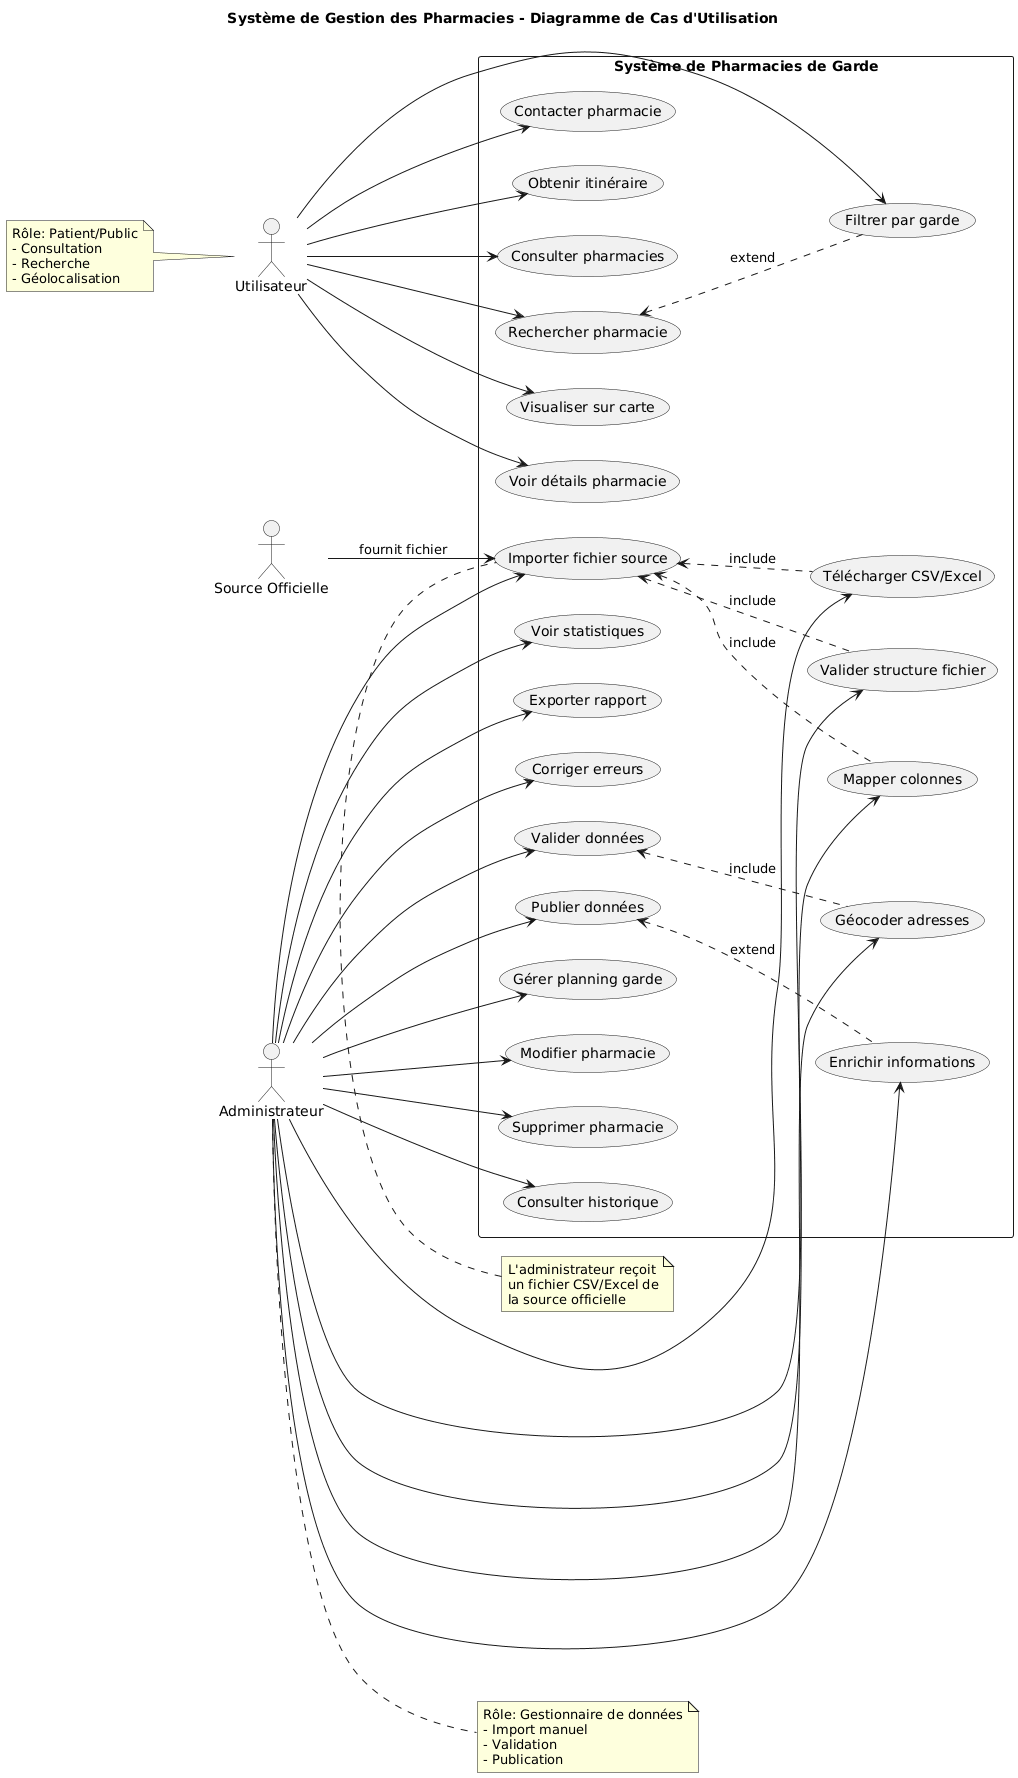
\includegraphics[width=0.82\textwidth,keepaspectratio]{usecasediag}
    \caption{Diagramme de cas d'utilisation détaillé\\ \small Source : Auteur}
    \label{fig:use-case-detaille}
\end{figure}

\section{Conclusion}

Au terme de cette analyse, les acteurs, les besoins et les règles de gestion de PharmacieConnect sont
posés. Il en ressort que la plateforme doit concilier consultation rapide, administration encadrée, qualité
des données et traçabilité. Le chapitre suivant traduit ces besoins en architecture, modèle de données,
diagrammes et mécanismes de sécurité.

\clearpage

\chapter{Conception}
\label{ch:conception}
\minitoc
\clearpage

\section{Introduction}

Concevoir PharmacieConnect a d'abord consisté à répartir les besoins fonctionnels exposés au chapitre
précédent entre les différentes briques de la solution. Le backend FastAPI assume les règles métier, la
sécurité, les imports et l'accès aux données. L'interface React/Vite prend en charge les opérations
d'administration, pendant que l'application Expo/React Native reste dédiée au parcours citoyen. Ce découpage
a été choisi pour ne pas dupliquer les règles sensibles dans les clients et pour conserver une architecture
plus simple à tester et à faire évoluer.

\section{Architecture globale}

L'architecture de PharmacieConnect place FastAPI comme point de passage unique entre les interfaces et les
données. Le tableau de bord React/Vite utilise cette API pour les opérations de gestion, alors que
l'application Expo/React Native l'utilise principalement pour la recherche, les gardes, les médicaments et le
compte utilisateur. Cette organisation évite que les règles de validation, d'audit et de restriction régionale
soient dupliquées dans les clients, comme l'illustre la Figure~\ref{fig:architecture-globale}.

\begin{figure}[H]
    \centering
    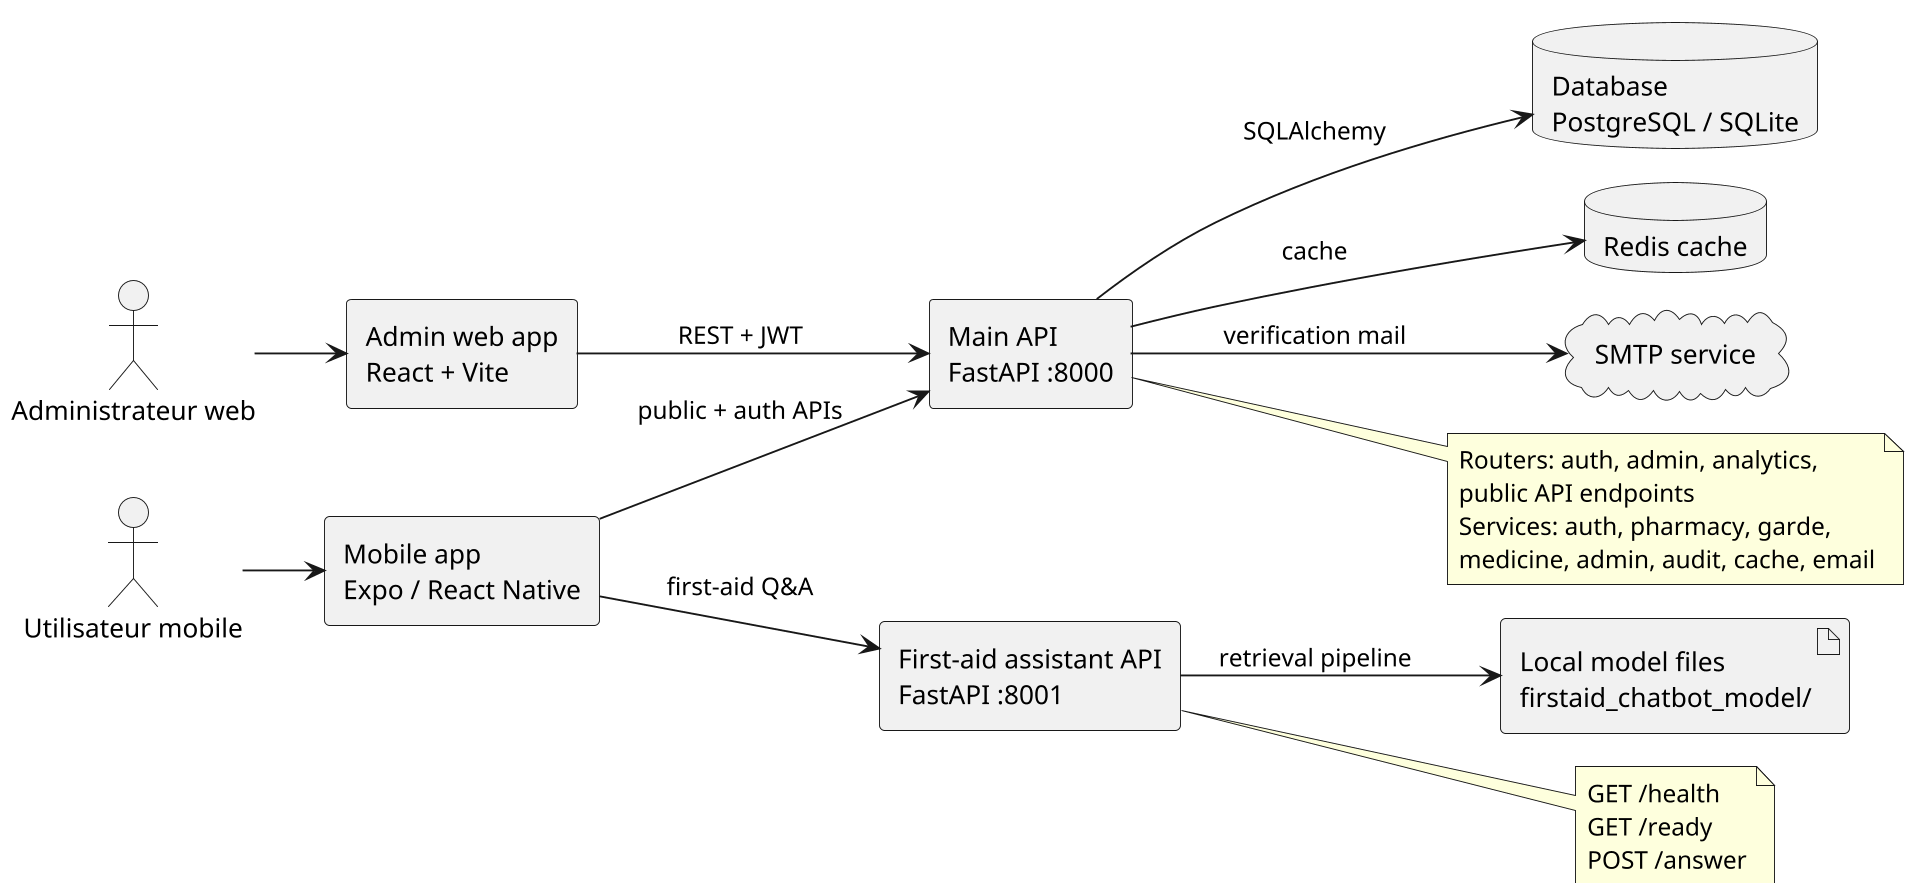
\includegraphics[width=0.95\textwidth]{plantuml/architecture_globale}
    \caption{Architecture globale de PharmacieConnect\\ \small Source : Auteur}
    \label{fig:architecture-globale}
\end{figure}

L'application mobile utilise principalement les endpoints publics de consultation, les routes liées au
compte utilisateur et l'API de l'assistant. Le panneau d'administration s'appuie sur des endpoints
protégés pour les opérations de gestion : ajout, mise à jour et retrait d'entrées, import CSV, consultation
des indicateurs et audit. Le backend devient ainsi la couche commune qui applique les règles métier avant toute
lecture ou écriture persistante.

\section{Backend FastAPI}

Dans le projet, FastAPI n'a pas été utilisé uniquement pour exposer des routes REST \cite{fastapi}. Il
constitue la couche qui relie les modules essentiels de PharmacieConnect : authentification, pharmacies,
gardes, médicaments, imports CSV, audit, indicateurs et assistant de premiers secours. Les routes restent
séparées des services métier afin que les règles de validation, les restrictions régionales et les accès à
la base via SQLAlchemy soient centralisés dans le backend plutôt que dispersés entre les interfaces. Le
Tableau~\ref{tab:backend-organisation} présente cette organisation.

\begin{table}[H]
    \centering
    \caption{Organisation du backend\\ \small Source : Auteur}
    \label{tab:backend-organisation}
    \begin{tabular}{L{4cm}L{9cm}}
        \toprule
        \textbf{Élément} & \textbf{Rôle} \\
        \midrule
        \texttt{main.py} & Initialisation de l'application FastAPI, middlewares, migrations au démarrage et endpoints publics. \\
        \texttt{routers/} & Routes d'authentification, d'administration et d'indicateurs. \\
        \texttt{services/} & Logique métier liée à l'authentification, aux pharmacies, aux gardes, aux médicaments, à l'audit et au cache. \\
        \texttt{models.py} & Modèles SQLAlchemy représentant les tables principales. \\
        \texttt{schemas.py} & Schémas Pydantic utilisés pour valider les entrées et structurer les sorties. \\
        \texttt{migrations/} & Scripts SQL permettant de faire évoluer le schéma de la base. \\
        \texttt{events/} & Bus d'événements interne et écouteurs associés. \\
        \bottomrule
    \end{tabular}
\end{table}

Le traitement d'une requête suit généralement le même parcours. Le client appelle une route FastAPI ; la
route vérifie les paramètres et l'utilisateur courant ; le service métier applique ensuite les règles
nécessaires avant l'accès à la base via SQLAlchemy.

\section{Tableau de bord React/Vite}

Côté administration, React et Vite ont été retenus pour construire une interface que l'on peut faire évoluer
page par page \cite{react,vite}. Dans notre cas, cette modularité est utile parce que le tableau de bord ne
sert pas seulement à afficher des informations : il doit aussi permettre de corriger les registres,
d'importer des fichiers, de vérifier des indicateurs et de suivre les actions sensibles (voir
Tableau~\ref{tab:admin-organisation}).

\begin{table}[H]
    \centering
    \caption{Organisation de l'administration web\\ \small Source : Auteur}
    \label{tab:admin-organisation}
    \begin{tabular}{L{4cm}L{9cm}}
        \toprule
        \textbf{Élément} & \textbf{Rôle} \\
        \midrule
        \texttt{src/pages/} & Pages principales du tableau de bord : pharmacies, gardes, médicaments, carte, audit, paramètres et gestion. \\
        \texttt{src/components/} & Composants d'interface, tableaux, formulaires, modales, cartes statistiques et éléments de layout. \\
        \texttt{src/context/} & Gestion de l'authentification, de la langue et de certains états globaux. \\
        \texttt{src/lib/api.js} & Client Axios responsable des appels backend et de l'injection du jeton JWT. \\
        \texttt{src/styles/} & Styles et utilitaires liés à la présentation de l'interface. \\
        \bottomrule
    \end{tabular}
\end{table}

Cette organisation évite de mélanger l'affichage avec la logique d'accès aux données. Le client API ajoute
le jeton d'accès aux requêtes protégées et prend en charge le renouvellement de session lorsque le jeton
expire.

\section{Application mobile Expo/React Native}

Pour la partie mobile, Expo et React Native ont été choisis afin de développer rapidement des écrans centrés
sur le parcours citoyen \cite{expo,reactnative}. L'organisation retenue suit les actions que l'utilisateur
réalise réellement dans l'application : chercher une pharmacie, ouvrir la carte, choisir une date de garde,
consulter un médicament, gérer son compte ou accéder à l'assistant de premiers secours, comme indiqué dans
le Tableau~\ref{tab:mobile-organisation}.

\begin{table}[H]
    \centering
    \caption{Organisation de l'application mobile\\ \small Source : Auteur}
    \label{tab:mobile-organisation}
    \begin{tabular}{L{4cm}L{9cm}}
        \toprule
        \textbf{Élément} & \textbf{Rôle} \\
        \midrule
        \texttt{screens/} & Écrans de l'application : accueil, carte, calendrier, médicaments, connexion, inscription, vérification email et paramètres. \\
        \texttt{components/} & Composants réutilisables comme les cartes de pharmacies, modales, sélecteurs et éléments RTL. \\
        \texttt{config/api.js} & Configuration de l'URL backend et des appels API. \\
        \texttt{utils/} & Fonctions utilitaires pour les données, les couleurs, le thème, le logging et la gestion RTL. \\
        \texttt{locales/} & Fichiers de traduction français, anglais et arabe. \\
        \bottomrule
    \end{tabular}
\end{table}

Des contextes React Native partagent certaines informations entre les écrans, comme l'authentification,
la langue, le thème, les favoris, les filtres et les notifications. Cette approche évite de répéter la même
logique dans plusieurs parties de l'application.

\section{Modèle de données}

Le modèle de données a été construit avec SQLAlchemy \cite{sqlalchemy} à partir des objets réellement
manipulés par l'application. Le tableau suivant ne cherche donc pas à donner une définition générale de ces
entités ; il précise plutôt comment PharmacieConnect organise les comptes, les pharmacies, les gardes, les
médicaments, les sessions, les tentatives de connexion, les recherches et l'audit, comme le détaille le
Tableau~\ref{tab:entites-donnees}.

\begin{longtable}{L{4cm}L{10cm}}
    \caption{Entités principales du modèle de données\\ \small Source : Auteur}\label{tab:entites-donnees}\\
    \toprule
    \textbf{Entité} & \textbf{Description} \\
    \midrule
    \endfirsthead
    \toprule
    \textbf{Entité} & \textbf{Description} \\
    \midrule
    \endhead
    \texttt{Utilisateur} & Compte utilisateur de l'application mobile avec email, mot de passe, statut actif et vérification email. \\
    \texttt{Administrateur} & Compte de gestion avec rôle, statut, informations de profil et périmètre régional éventuel. \\
    \texttt{RefreshToken} & Jeton de rafraîchissement permettant de prolonger une session selon les règles de sécurité. \\
    \texttt{LoginAttempt} & Tentative de connexion utilisée pour suivre les succès et les échecs d'authentification. \\
    \texttt{Pharmacie} & Données d'une pharmacie : nom, adresse, téléphone, gouvernorat, latitude, longitude et référence OSM éventuelle. \\
    \texttt{GardeSchedule} & Planning de garde avec date, pharmacie, horaire, ville, gouvernorat, type de garde et notes. \\
    \texttt{Medicine} & Catalogue de médicaments avec code PCT, nom commercial, prix public, tarif de référence, remboursement, DCI et AP. \\
    \texttt{AuditLog} & Trace des actions importantes avec acteur, cible, statut, adresse IP et détails. \\
    \texttt{SearchEvent} & Événements de recherche utilisés pour alimenter les statistiques et les indicateurs. \\
    \bottomrule
\end{longtable}

\section{Diagramme de classes}

Le diagramme de classes décrit le modèle de données réel de PharmacieConnect, fidèle aux entités persistées
par le backend via SQLAlchemy. Comme le montre la Figure~\ref{fig:class-diagram}, il distingue les comptes
(\texttt{Administrateur}, \texttt{Utilisateur}) et leurs mécanismes de sécurité, les pharmacies et leurs
plannings de garde, les médicaments, ainsi que la traçabilité assurée par les journaux d'audit.

\begin{figure}[H]
    \centering
    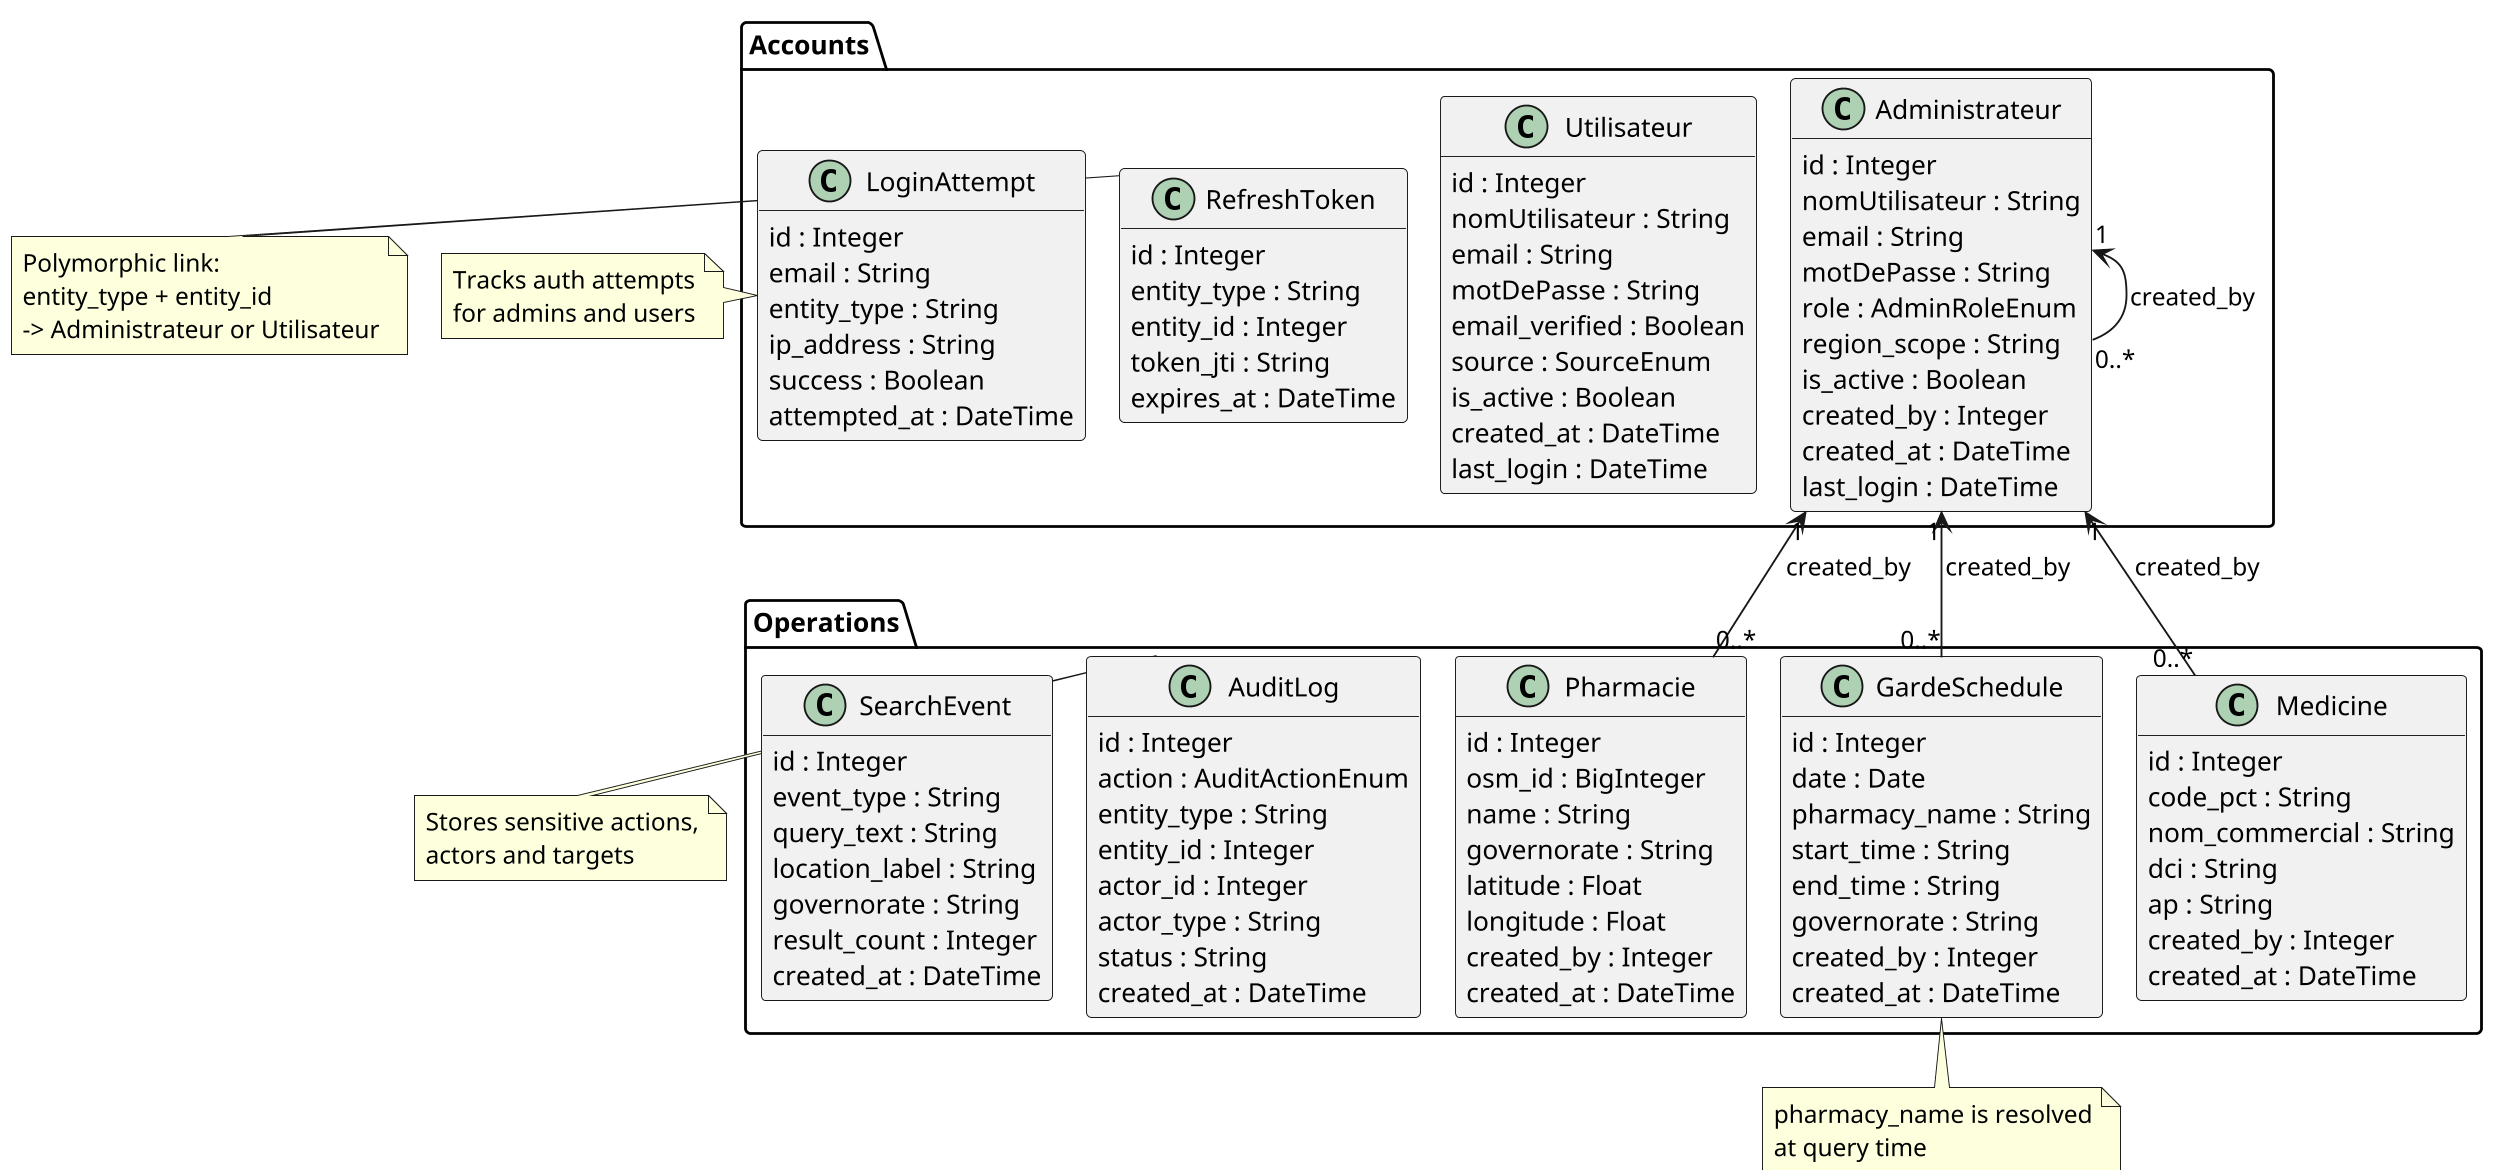
\includegraphics[width=0.95\textwidth]{plantuml/class_diagram}
    \caption{Diagramme de classes\\ \small Source : Auteur}
    \label{fig:class-diagram}
\end{figure}

La Figure~\ref{fig:class-diagram} met en évidence les entités centrales du modèle. Les deux types de comptes,
\texttt{Administrateur} (dont le \texttt{role} est typé par \texttt{AdminRoleEnum} et complété d'un
\texttt{region\_scope} pour la délégation régionale) et \texttt{Utilisateur}, partagent les mécanismes de
session : \texttt{RefreshToken} et \texttt{LoginAttempt} y sont rattachés par un lien polymorphe
(\texttt{entity\_type} + \texttt{entity\_id}). L'\texttt{Administrateur} est l'auteur des données qu'il
saisit : les attributs \texttt{created\_by} relient \texttt{Pharmacie}, \texttt{GardeSchedule} et
\texttt{Medicine} au compte qui les a créés, tandis que \texttt{AuditLog} référence son auteur via
\texttt{actor\_id}. La \texttt{Pharmacie} et le \texttt{GardeSchedule} ne sont toutefois pas liés par une
clé étrangère directe : la correspondance s'effectue par le nom de la pharmacie au moment de la requête
(\texttt{pharmacy\_name}). Enfin, \texttt{SearchEvent} conserve les événements de recherche utiles aux
indicateurs. L'assistant de premiers secours n'apparaît pas dans ce schéma, car il fonctionne comme un
service de récupération sans état, sans persistance de conversation. Cette organisation traduit la
séparation des responsabilités : des comptes distincts, des données métier centralisées autour de la
pharmacie et une traçabilité systématique des actions sensibles.

\section{Diagrammes de séquence}

Les diagrammes de séquence retenus décrivent deux parcours critiques du projet. Le premier, présenté dans la
Figure~\ref{fig:sequence-auth}, montre comment une session est créée puis contrôlée à travers les jetons JWT.
Le second, donné par la Figure~\ref{fig:sequence-search}, détaille la recherche d'une pharmacie, depuis la
saisie ou la géolocalisation côté mobile jusqu'au filtrage effectué par le backend. Ces
deux scénarios ont été choisis parce qu'ils concentrent les principaux échanges entre les clients, les
services métier et la base de données.

\begin{figure}[H]
    \centering
    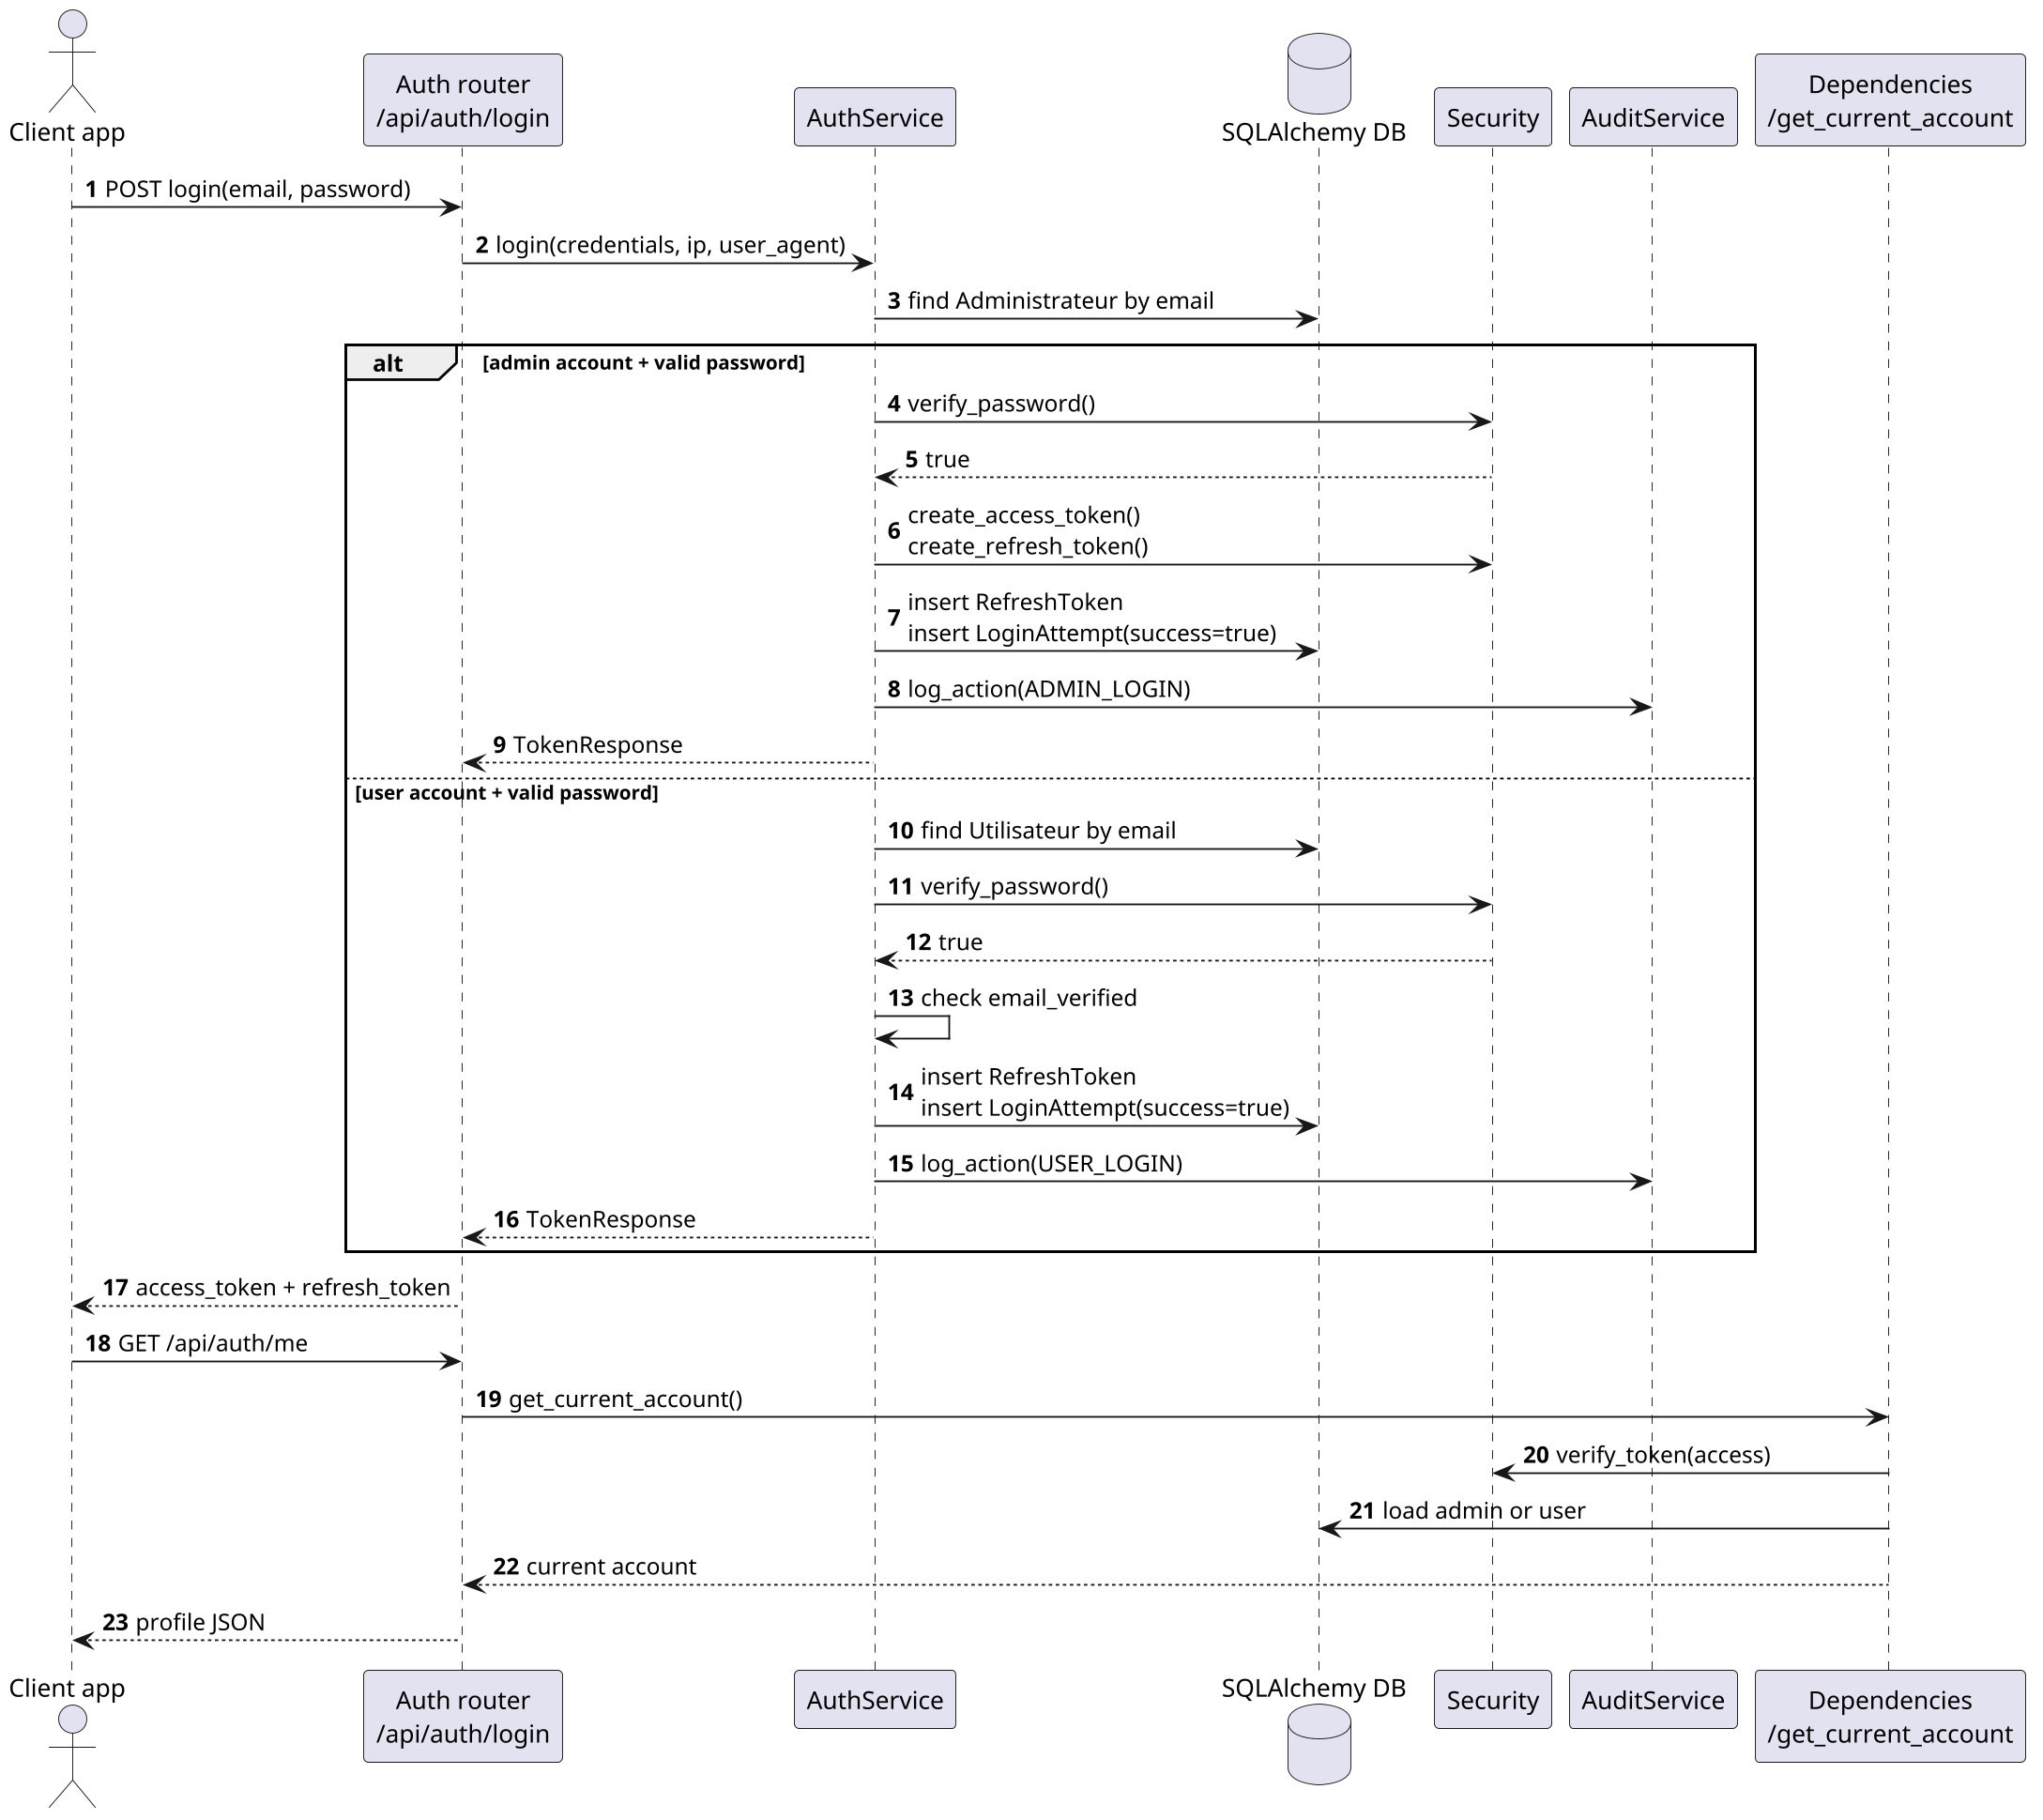
\includegraphics[width=0.95\textwidth]{plantuml/sequence_auth_jwt}
    \caption{Diagramme de séquence : authentification JWT\\ \small Source : Auteur}
    \label{fig:sequence-auth}
\end{figure}

\begin{figure}[H]
    \centering
    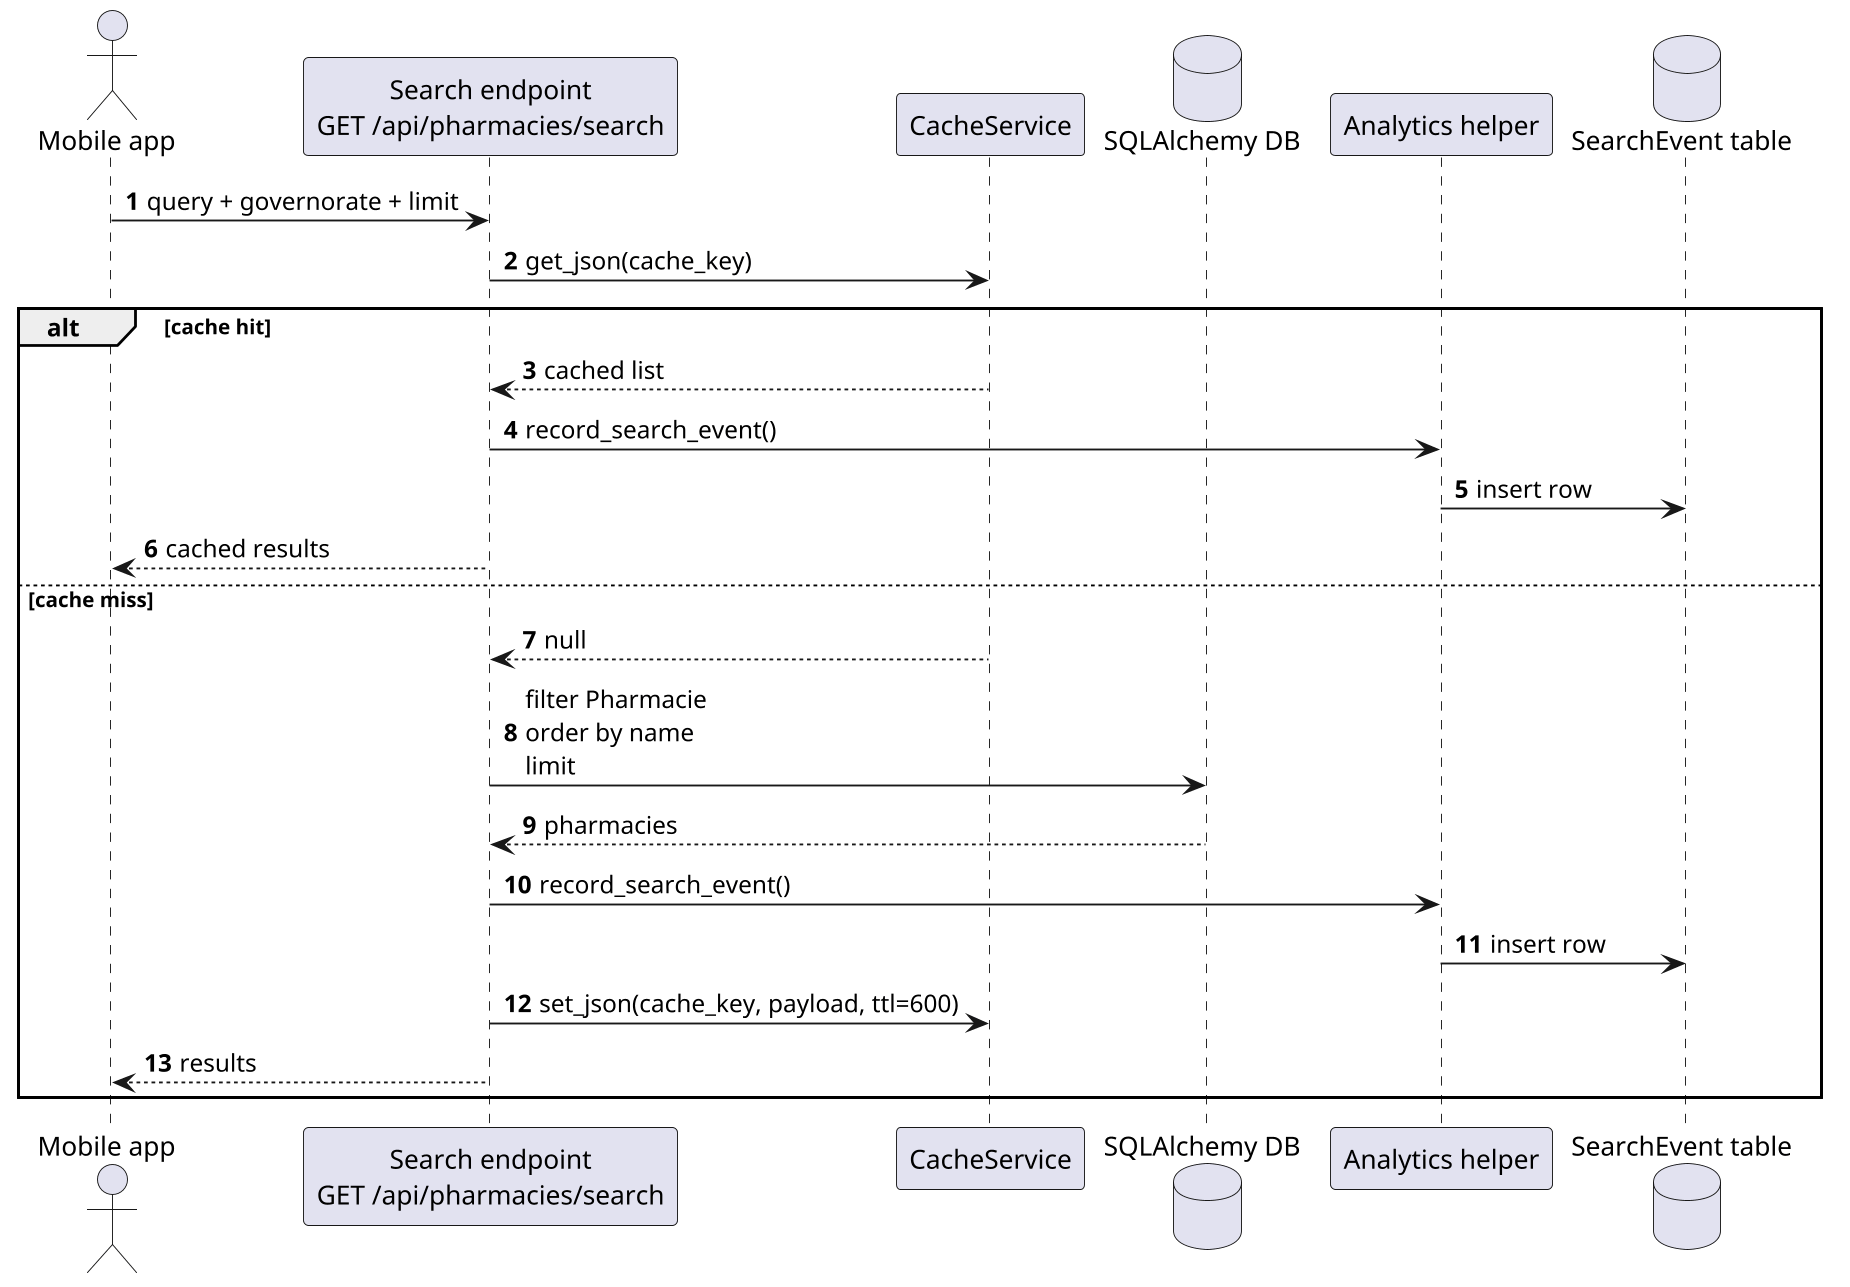
\includegraphics[width=0.95\textwidth]{plantuml/sequence_pharmacy_search}
    \caption{Diagramme de séquence : recherche d'une pharmacie\\ \small Source : Auteur}
    \label{fig:sequence-search}
\end{figure}

\section{Diagramme d'activité}

Le diagramme d'activité détaille le traitement d'un import CSV. Ce scénario est important, car il regroupe
plusieurs règles sensibles : contrôle du fichier, validation des colonnes, vérification des lignes,
enregistrement des données valides, rejet des lignes incorrectes et journalisation du résultat
(voir Figure~\ref{fig:activity-import-csv}).

\begin{figure}[H]
    \centering
    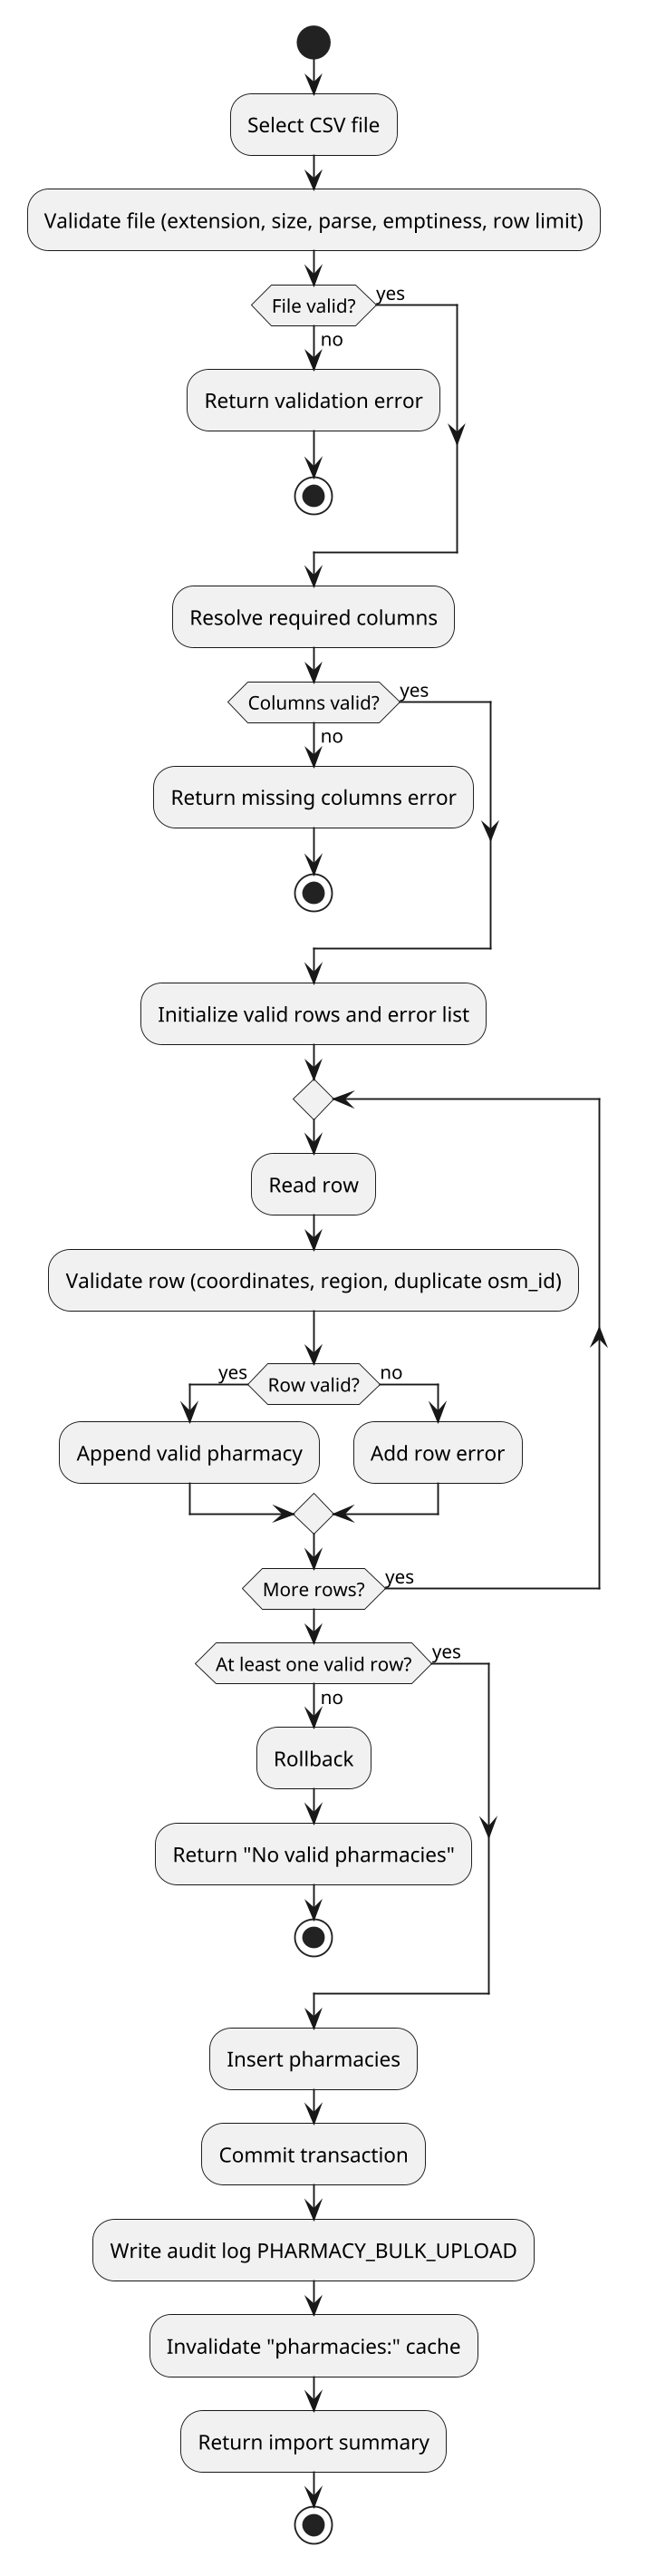
\includegraphics[height=0.85\textheight,keepaspectratio]{plantuml/activity_csv_import}
    \caption{Diagramme d'activité : import CSV contrôlé\\ \small Source : Auteur}
    \label{fig:activity-import-csv}
\end{figure}

\section{Diagramme de composants et de déploiement}

Les diagrammes de composants et de déploiement complètent la vision technique. Le premier, représenté dans la
Figure~\ref{fig:component-diagram}, décrit les modules logiciels, tandis que le second, illustré par la
Figure~\ref{fig:deployment-diagram}, présente la répartition logique entre les clients, le serveur backend,
la base de données et la configuration.

\begin{figure}[H]
    \centering
    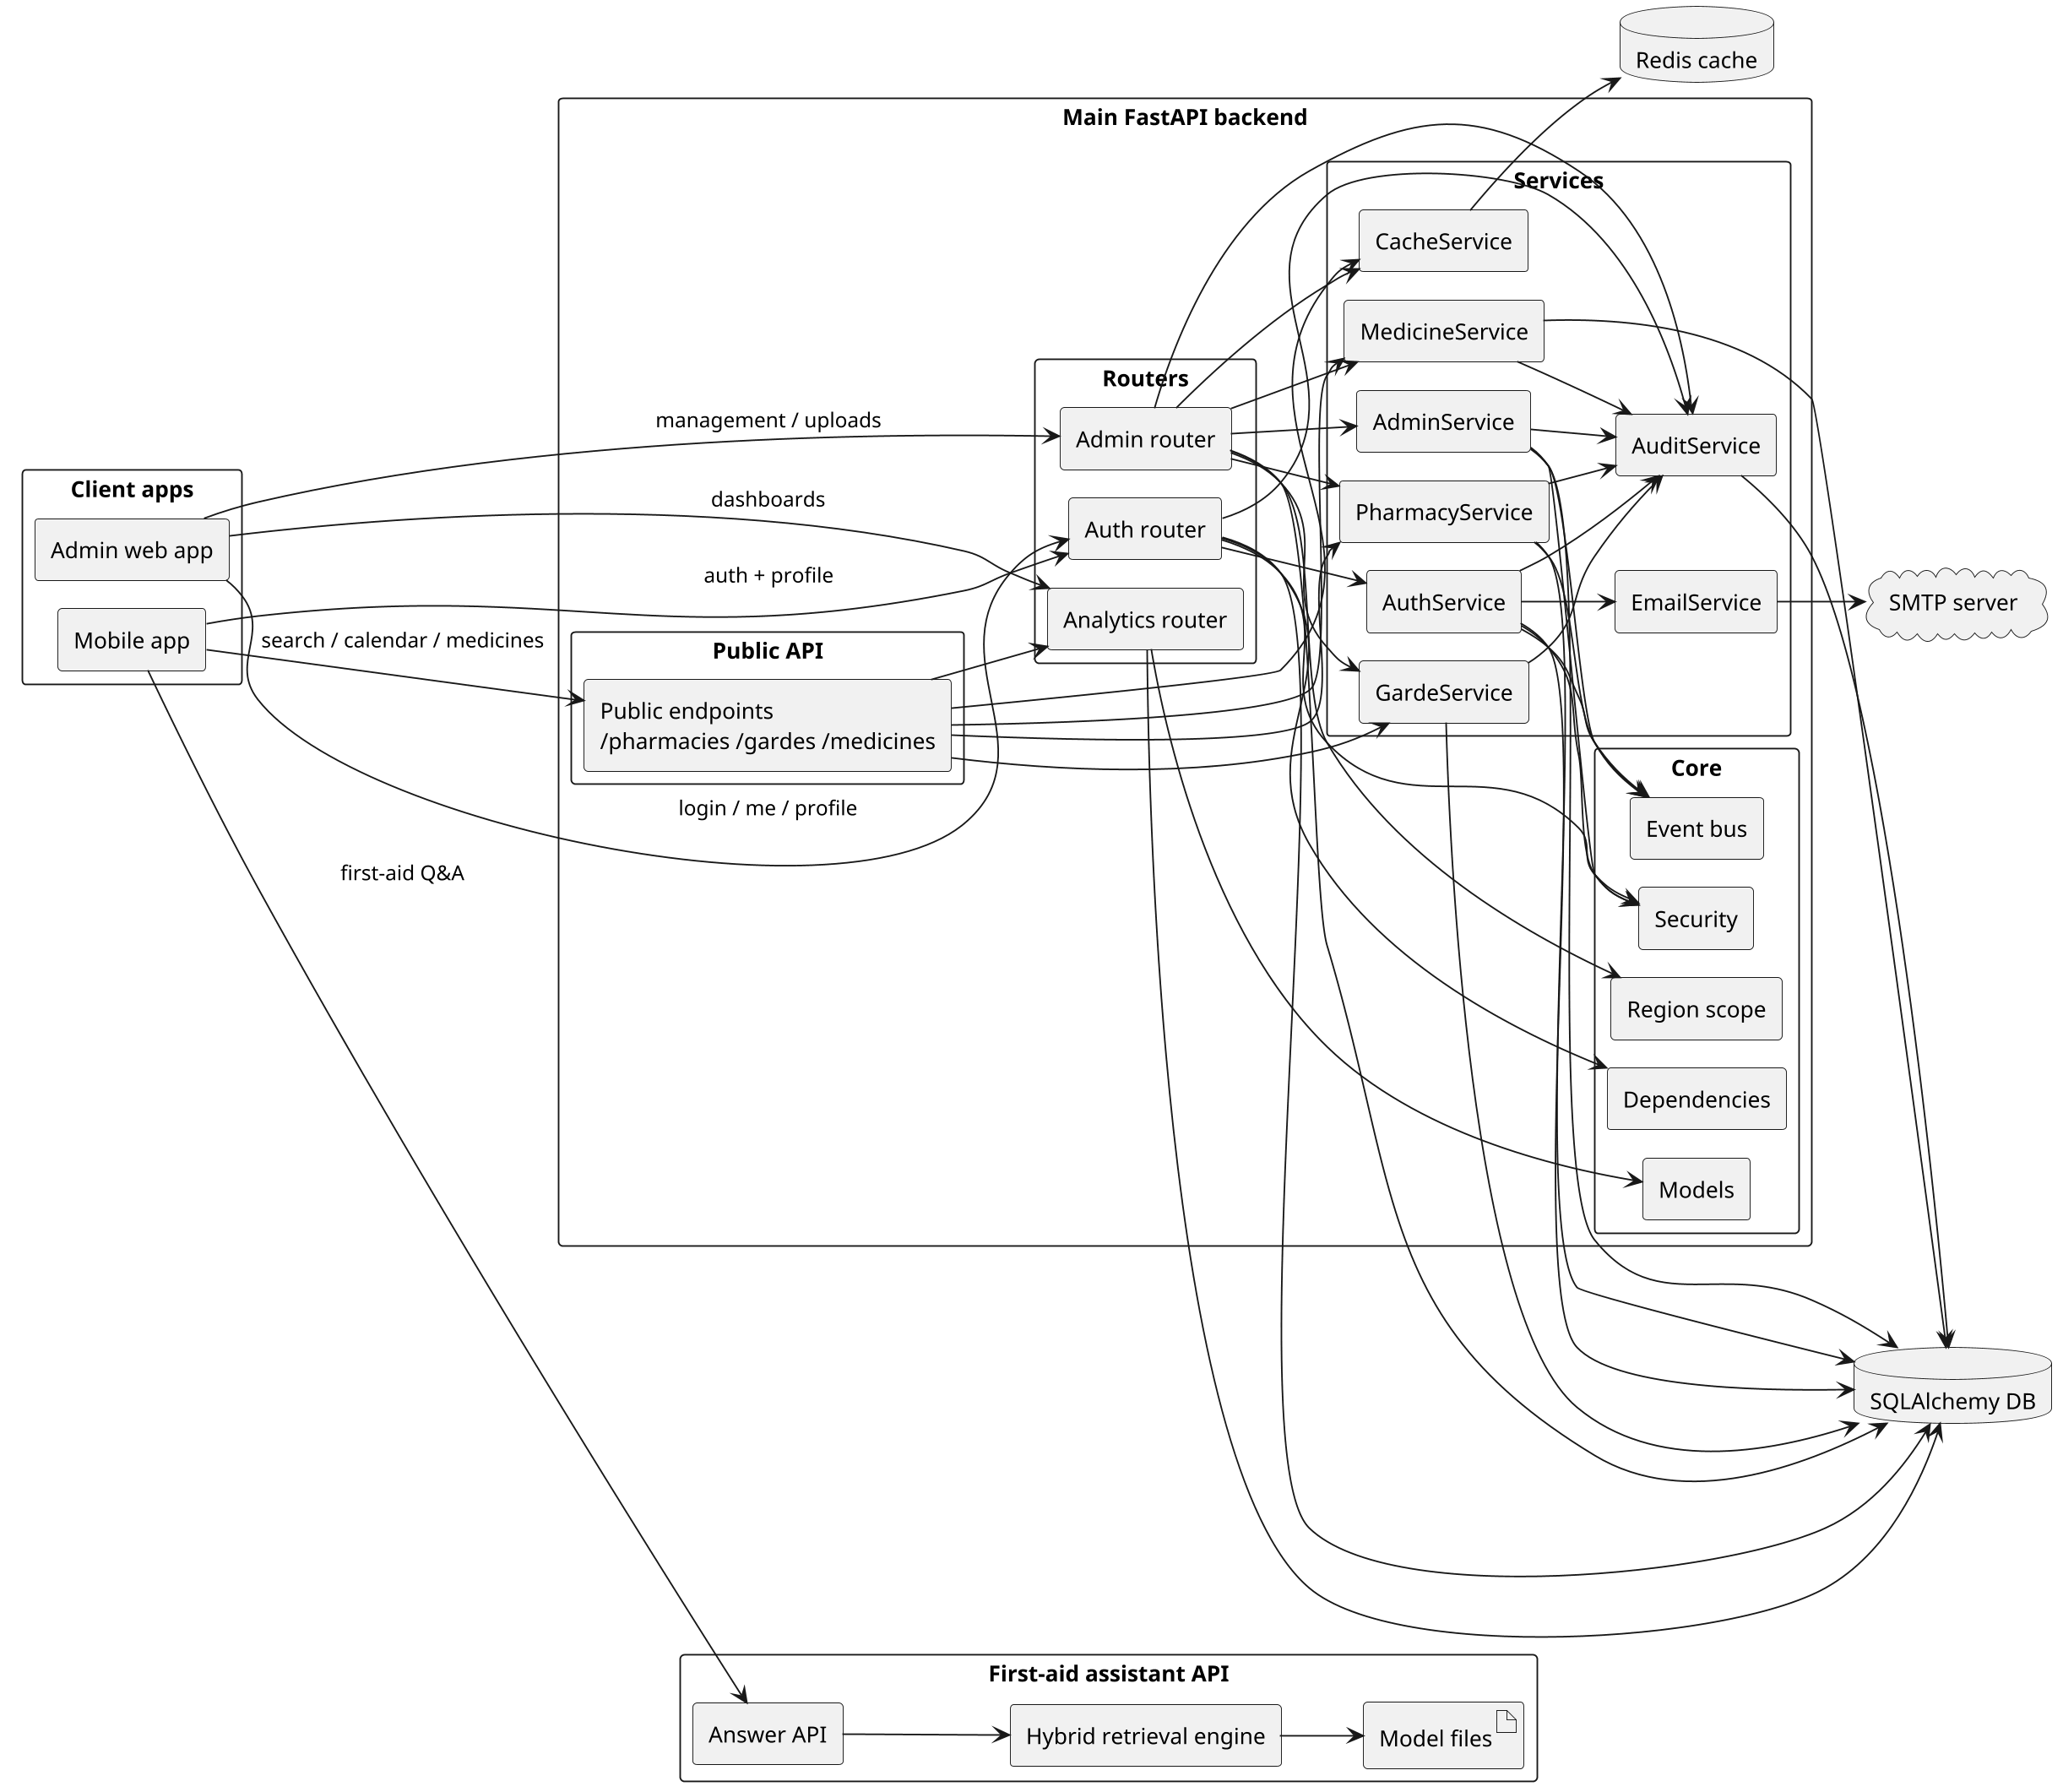
\includegraphics[width=0.95\textwidth]{plantuml/component_diagram}
    \caption{Diagramme de composants\\ \small Source : Auteur}
    \label{fig:component-diagram}
\end{figure}

\begin{figure}[H]
    \centering
    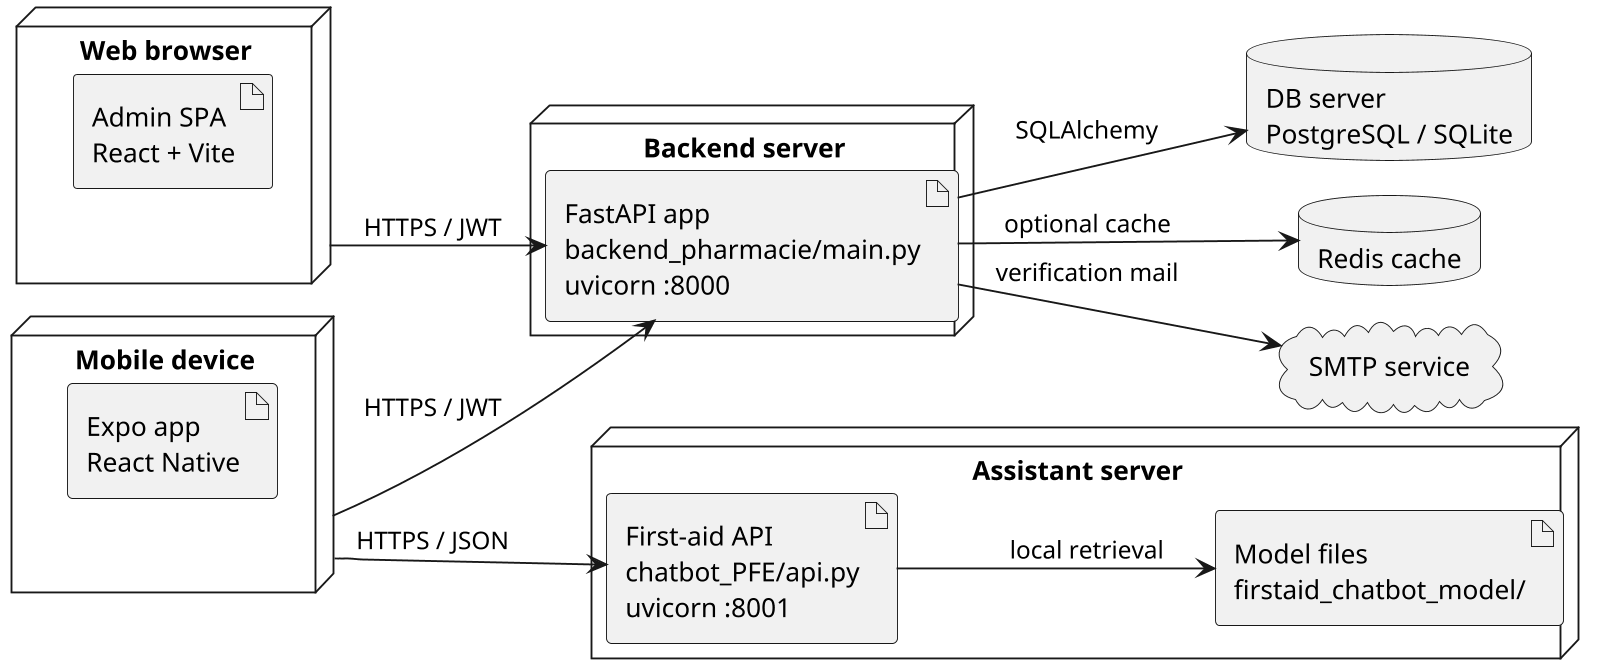
\includegraphics[width=0.95\textwidth]{plantuml/deployment_diagram}
    \caption{Diagramme de déploiement\\ \small Source : Auteur}
    \label{fig:deployment-diagram}
\end{figure}

\section{Sécurité}
\label{sec:securite}

La sécurité de PharmacieConnect est appliquée côté backend afin que les règles ne dépendent pas uniquement
de l'affichage dans les interfaces. Les routes d'administration exigent un jeton JWT valide, puis vérifient le
rôle du compte connecté. Pour les assistants, le contrôle ne s'arrête pas au rôle : le périmètre régional est
également vérifié avant toute création, modification ou suppression. Cette approche, alignée avec les
recommandations OWASP pour la protection des API~\cite{owasp}, protège particulièrement les imports CSV, les
gardes, les médicaments et les journaux d'audit.

\subsection{Gestion des sessions par jetons JWT}

La gestion des sessions dans PharmacieConnect distingue deux jetons aux durées de vie volontairement
différentes. À la connexion, le backend émet un jeton d'accès valable 15~minutes par défaut, signé avec
HS256, et un jeton de rafraîchissement valable 7~jours. Le premier accompagne chaque requête
protégée dans l'en-tête \texttt{Authorization: Bearer} ; sa courte durée limite les conséquences
d'une interception. Le second est conservé en base dans l'entité \texttt{RefreshToken} et effacé
lors de la déconnexion explicite, ce qui permet de renouveler la session active sans laisser
le jeton d'accès circuler au-delà de sa fenêtre autorisée.

La validation de ces jetons est prise en charge exclusivement par le backend à chaque appel
protégé : déléguer ce contrôle à l'interface cliente serait insuffisant, car tout appel direct à
l'API contournerait alors les vérifications \cite{jwt}.

\subsection{Contrôle d'accès basé sur les rôles (\gls{rbac})}

PharmacieConnect organise les accès administratifs selon trois rôles : \texttt{super\_admin},
\texttt{admin} et \texttt{assistant}. Chaque endpoint protégé évalue le rôle du demandeur avant d'exécuter
l'opération. Pour le rôle \texttt{assistant}, un deuxième filtre s'applique : l'attribut
\texttt{region\_scope} limite les actions au périmètre régional autorisé. Toute tentative d'opération hors
de ce périmètre est rejetée même si le jeton d'accès est valide. Cette combinaison rôle\,/\,périmètre répond
directement au besoin de délégation régionale : plusieurs assistants peuvent coexister sans modifier les
données qui ne relèvent pas de leur zone.

\subsection{Hachage des mots de passe}

Le projet a retenu bcrypt via Passlib pour protéger les mots de passe des administrateurs et des
utilisateurs mobiles. Chaque empreinte est produite avec un sel unique généré à l'enregistrement :
deux comptes utilisant le même mot de passe donnent des empreintes différentes, ce qui empêche
toute comparaison directe entre entrées. Le facteur de coût est réglé pour que la vérification
lors de la connexion reste imperceptible pour l'utilisateur, tout en rendant une attaque par
volume prohibitivement longue. La comparaison à la connexion s'opère uniquement sur les empreintes
stockées ; le mot de passe en clair n'est jamais conservé en base \cite{passlib_bcrypt}.

\subsection{Validation des entrées avec Pydantic}

Avant qu'une donnée entrante n'atteigne la couche service, un schéma Pydantic la valide
intégralement. Pour PharmacieConnect, cela concerne notamment les formats d'email des comptes,
les plages de coordonnées des pharmacies (latitude bornée entre $-90$ et $90$, longitude entre
$-180$ et $180$), les dates des plannings de garde, les codes PCT des médicaments et la taille
maximale des fichiers CSV importés. Regrouper ces contrôles dans les schémas évite de les
répliquer dans chaque route et intercepte les données malformées avant tout accès à la base \cite{pydantic}.

\subsection{Politique \gls{cors} et hôtes autorisés}

Le backend déclare explicitement les origines autorisées via les variables d'environnement de configuration
CORS. Toute origine non prévue par la configuration ne doit pas accéder aux routes depuis un navigateur.
En complément, \texttt{TrustedHostMiddleware} inspecte l'en-tête d'hôte de chaque requête et bloque celles
dont l'hôte n'est pas inscrit dans \texttt{TRUSTED\_HOSTS}. Ces paramètres sont externalisés afin d'adapter
la configuration entre le développement local et un déploiement en production.

\subsection{Traçabilité et journalisation des actions}

Deux mécanismes de traçabilité coexistent dans PharmacieConnect. La table \texttt{LoginAttempt} enregistre
les tentatives de connexion avec leur statut, l'adresse IP source et l'horodatage. En parallèle, le service
\texttt{AuditService} journalise les opérations administratives significatives : ajout, mise à jour et
retrait d'entités, imports CSV et changements de droits. Chaque entrée d'audit identifie l'acteur,
décrit l'opération, référence la cible et indique le résultat. Cette granularité permet de reconstituer
l'historique des modifications apportées aux données de la plateforme.

\subsection{Sécurité du déploiement}

Pour un déploiement en production, les mesures complémentaires recommandées sont :

\begin{itemize}
    \item forcer \textbf{HTTPS} sur toutes les communications et rediriger le trafic HTTP ;
    \item utiliser une \texttt{SECRET\_KEY} aléatoire d'au moins 256 bits, distincte entre
    les environnements de développement et de production ;
    \item remplacer SQLite par \textbf{PostgreSQL} pour une gestion robuste des connexions
    concurrentes ;
    \item activer le cache \textbf{Redis} pour réduire la pression sur la base de données et
    limiter les requêtes répétitives.
\end{itemize}

\section{Justification des choix techniques}

Le Tableau~\ref{tab:choix-techniques} justifie les principaux choix techniques retenus pour le projet.

\begin{longtable}{L{4cm}L{10cm}}
    \caption{Justification des choix techniques\\ \small Source : Auteur}\label{tab:choix-techniques}\\
    \toprule
    \textbf{Choix} & \textbf{Justification} \\
    \midrule
    \endfirsthead
    \toprule
    \textbf{Choix} & \textbf{Justification} \\
    \midrule
    \endhead
    FastAPI & Retenu pour concentrer les endpoints publics et protégés dans un backend testable, avec validation des requêtes et documentation API utile pendant les essais \cite{fastapi}. \\
    React et Vite & Retenus pour structurer le tableau de bord par pages fonctionnelles : pharmacies, gardes, médicaments, audit et paramètres \cite{react,vite}. \\
    Expo et React Native & Retenus pour réaliser les écrans mobiles liés au parcours citoyen : recherche, carte, calendrier, médicaments, profil et assistant \cite{expo,reactnative}. \\
    SQLAlchemy & Retenu pour représenter les entités métier du projet et garder l'accès aux tables dans les services backend \cite{sqlalchemy}. \\
    SQLite et PostgreSQL & SQLite facilite la validation locale, tandis que PostgreSQL reste plus adapté à un déploiement avec connexions concurrentes \cite{postgresql}. \\
    JWT & Retenu pour séparer un jeton d'accès court et un jeton de rafraîchissement, afin de protéger les routes administratives et les comptes utilisateurs \cite{jwt}. \\
    CSV & Retenu comme format d'import pragmatique pour les pharmacies, les gardes et les médicaments, avec validation des colonnes et retour des erreurs. \\
    \bottomrule
\end{longtable}

\section{Conclusion}

L'ensemble de cette conception offre une base cohérente pour passer à la réalisation de PharmacieConnect.
Les règles sensibles demeurent côté backend, chaque interface se consacre à son propre parcours et les
données métier s'organisent autour des pharmacies, des gardes, des médicaments et de l'audit. Une telle
séparation facilite la maîtrise des évolutions futures : ajout d'une règle d'import, création d'un rôle
administratif ou perfectionnement de l'assistant de premiers secours. Le chapitre qui suit fait le pont
entre cette conception, la réalisation technique et la validation de la solution.

\clearpage

\chapter{Réalisation et tests}
\label{ch:realisation-tests}
\minitoc
\clearpage

\section{Introduction}

Après la conception, cette partie décrit la réalisation concrète de PharmacieConnect. Elle présente
l'environnement de travail, les technologies utilisées, l'organisation du dépôt et les principales
fonctionnalités développées dans le backend, le tableau de bord administrateur et l'application mobile. La
fin du chapitre est consacrée à l'intégration, à la configuration, aux tests et aux difficultés rencontrées.

\section{Environnement matériel et logiciel}

Le développement de PharmacieConnect a mobilisé plusieurs outils, car le projet combine un backend, une
interface web d'administration et une application mobile.

\begin{table}[H]
    \centering
    \caption{Environnement de développement}
    \begin{tabular}{L{5cm}L{8cm}}
        \toprule
        \textbf{Élément} & \textbf{Description} \\
        \midrule
        Machine de développement & Ordinateur portable Intel Core i7-8750H, 12 threads, 16 Go RAM, stockage local 343 Go. \\
        Système d'exploitation & Linux 6.17 x86\_64. \\
        Éditeur de code & Visual Studio Code. \\
        Backend & Python, FastAPI, Uvicorn, SQLAlchemy, Pydantic, Pytest \\
        Administration web & Node.js, React, Vite, React Router, Axios, Tailwind CSS \\
        Application mobile & Expo, React Native, React Navigation, i18next \\
        Base de données & SQLite en développement local, PostgreSQL selon la configuration \\
        Outils de test & Pytest, Jest, build Vite et tests fonctionnels manuels \\
        \bottomrule
    \end{tabular}
\end{table}

\section{Technologies utilisées}

Les choix techniques découlent directement des besoins du projet. Le backend devait fournir des API
claires et sécurisées. L'administration nécessitait une interface web capable de gérer les données depuis
un navigateur. L'application mobile, de son côté, devait rester simple à utiliser tout en intégrant la
recherche, la carte et la consultation des gardes.

\begin{longtable}{L{4cm}L{10cm}}
    \caption{Technologies utilisées dans le projet}\\
    \toprule
    \textbf{Technologie} & \textbf{Utilisation} \\
    \midrule
    \endfirsthead
    \toprule
    \textbf{Technologie} & \textbf{Utilisation} \\
    \midrule
    \endhead
    FastAPI & Développement de l'API REST, endpoints publics et endpoints protégés. \\
    SQLAlchemy & Modélisation des entités et accès à la base de données. \\
    Pydantic & Validation des données entrantes et structuration des réponses. \\
    JWT & Authentification, jetons d'accès et jetons de rafraîchissement. \\
    React & Construction de l'interface d'administration. \\
    Vite & Outil de développement et de build pour le tableau de bord administrateur. \\
    Axios & Communication entre le tableau de bord administrateur et l'API. \\
    Tailwind CSS & Mise en forme de l'interface d'administration. \\
    Expo & Développement et exécution de l'application mobile. \\
    React Native & Création des écrans et composants mobiles. \\
    i18next & Gestion de l'internationalisation. \\
    OpenStreetMap / Nominatim & Référence cartographique et géocodage lorsque l'enrichissement des coordonnées est nécessaire \cite{nominatim}. \\
    Pytest & Tests automatisés du backend \cite{pytest}. \\
    Jest & Tests automatisés côté application mobile \cite{jest}. \\
    \bottomrule
\end{longtable}

\section{Organisation du dépôt}

Le projet est regroupé dans un même espace de travail. Cette structure a facilité l'intégration entre
l'API, le tableau de bord et l'application mobile, notamment lors des tests de communication entre les
clients et le backend.

\begin{table}[H]
    \centering
    \caption{Organisation générale du dépôt}
    \begin{tabular}{L{5.6cm}L{7.4cm}}
        \toprule
        \textbf{Dossier} & \textbf{Contenu} \\
        \midrule
        \path{backend_pharmacie/} & API FastAPI, modèles SQLAlchemy, services métier, migrations, sécurité et tests. \\
        \path{admin_pharmacie/} & Tableau de bord React/Vite destiné à l'administration. \\
        \begin{minipage}[t]{5.4cm}\ttfamily\small ouerkema-pharmacieconnect-\linebreak 4c94773cce7d/\end{minipage} & Application mobile Expo/React Native destinée aux utilisateurs finaux. \\
        \path{docs/} & Documentation technique liée à l'architecture, l'API, le backend, le web admin et le mobile. \\
        \bottomrule
    \end{tabular}
\end{table}

\section{Réalisation backend}

Le backend constitue la partie centrale de PharmacieConnect. Il reçoit les requêtes des deux interfaces,
applique les règles métier et interagit avec la base de données. Il regroupe également les mécanismes
d'authentification, de validation, d'audit et d'import.

\subsection{Endpoints publics}

Les endpoints publics répondent surtout aux besoins de l'application mobile. Ils donnent accès aux
informations de consultation sans passer par l'espace d'administration.

\begin{itemize}
    \item \texttt{GET /health} pour vérifier l'état du backend ;
    \item \texttt{GET /api/pharmacies} pour consulter les pharmacies avec pagination ;
    \item \texttt{GET /api/pharmacies/search} pour rechercher par texte ;
    \item \texttt{GET /api/pharmacies/nearby} pour rechercher les pharmacies proches d'une position GPS ;
    \item \texttt{GET /api/pharmacies/\{pharmacy\_id\}} pour consulter le détail d'une pharmacie ;
    \item \texttt{GET /api/gardes} pour consulter les gardes d'une date donnée ;
    \item \texttt{GET /api/medicines} pour rechercher dans le catalogue de médicaments ;
    \item \texttt{GET /api/medicines/\{code\_pct\}} pour consulter le détail d'un médicament.
\end{itemize}

Pour la recherche par proximité, l'API utilise les coordonnées GPS envoyées par le client. Elle calcule la
distance avec les pharmacies disponibles et retourne les résultats triés par distance.

\subsection{Authentification et sessions}

L'authentification est gérée côté backend afin de garder le contrôle sur les comptes et les autorisations.
Lorsqu'une connexion réussit, le serveur retourne un jeton d'accès et un jeton de rafraîchissement.

\begin{lstlisting}[caption={Structure simplifiée d'une réponse de connexion}]
{
  "access_token": "[jeton d'acces]",
  "refresh_token": "[jeton de rafraichissement]",
  "token_type": "bearer",
  "expires_in": 1800
}
\end{lstlisting}

Les routes protégées vérifient ensuite le jeton reçu et le rôle de l'utilisateur. Cette vérification est
réalisée côté serveur afin qu'un simple contrôle d'interface ne puisse pas être contourné.

\subsection{Services métier}

La logique principale est placée dans des services. Ce choix évite de concentrer trop de code dans les
routes et rend les traitements plus faciles à tester.

\begin{itemize}
    \item \texttt{AuthService} pour l'inscription, la connexion, la vérification email, le rafraîchissement et la déconnexion ;
    \item \texttt{PharmacyService} pour la gestion et l'import des pharmacies ;
    \item \texttt{GardeService} pour la gestion et l'import des plannings de garde ;
    \item \texttt{MedicineService} pour l'import, la recherche et la consultation des médicaments ;
    \item \texttt{AuditService} pour la journalisation des actions importantes ;
    \item \texttt{CacheService} pour l'utilisation du cache lorsque la configuration le permet.
\end{itemize}

\subsection{Imports CSV}

Les imports CSV ont été ajoutés pour éviter la saisie manuelle d'un grand nombre de lignes. Avant
l'enregistrement, le backend vérifie l'extension, la taille, les colonnes obligatoires, le format des
valeurs et les contraintes métier.

Lorsqu'une ligne est incorrecte, la réponse indique les informations nécessaires pour corriger le fichier.
Pour les médicaments, le code PCT sert d'identifiant pour mettre à jour un enregistrement existant au lieu
de créer un doublon.

\subsection{Audit et indicateurs}

Les actions sensibles sont enregistrées dans les journaux d'audit. Cela concerne notamment les
connexions, les échecs de connexion, les inscriptions, les créations administratives et les imports. Les
données statistiques alimentent le tableau de bord et donnent une vision synthétique de l'activité.

\section{Réalisation du tableau de bord administrateur}

Le tableau de bord administrateur rassemble les fonctions de gestion dans une interface web destinée aux
administrateurs et aux utilisateurs autorisés.

\subsection{Pages principales}

Les principales pages développées sont :

\begin{itemize}
    \item le tableau de bord pour les compteurs, indicateurs et activités récentes ;
    \item la page des pharmacies pour consulter, créer, modifier, supprimer et importer les pharmacies ;
    \item la page des gardes pour gérer les plannings de garde ;
    \item la page des médicaments pour importer et consulter le catalogue ;
    \item la carte pour visualiser les pharmacies géographiquement ;
    \item la page de management pour gérer les assistants et les autorisations ;
    \item la page des journaux d'audit pour consulter les actions enregistrées ;
    \item les pages de profil, paramètres, notifications et langues.
\end{itemize}

\subsection{Gestion des sessions côté administration}

Le tableau de bord utilise un client API centralisé. Ce client ajoute le jeton JWT aux requêtes protégées.
Si le jeton d'accès expire, il tente de renouveler la session. En cas d'échec, l'utilisateur est redirigé
vers la page de connexion.

\section{Réalisation application mobile}

L'application mobile correspond à la partie utilisée par le citoyen. Elle regroupe la recherche, la
consultation des gardes, la carte, le catalogue de médicaments et les paramètres.

\subsection{Recherche et détail des pharmacies}

Depuis l'écran d'accueil, l'utilisateur peut rechercher une pharmacie par texte et consulter les résultats.
La fiche de détail affiche les informations disponibles, comme le nom, l'adresse, le téléphone, le
gouvernorat et les coordonnées lorsque celles-ci existent.

\subsection{Carte et géolocalisation}

L'application peut demander l'autorisation d'utiliser la position de l'utilisateur. Cette position est
envoyée au backend afin de récupérer les pharmacies proches. La carte affiche ensuite les résultats sous
forme de marqueurs.

\subsection{Calendrier des gardes}

Le calendrier donne à l'utilisateur le choix d'une date et affiche les pharmacies de garde correspondantes.
Cette fonctionnalité répond au besoin principal du projet : trouver rapidement une pharmacie disponible à
une date précise.

\subsection{Catalogue de médicaments}

L'écran des médicaments prend en charge la recherche par nom commercial, DCI ou code PCT. La fiche de détail
affiche les informations présentes dans la base, comme le prix public, le tarif de référence et la catégorie
de remboursement.

\subsection{Paramètres, langues et thème}

L'application prend en charge le français, l'anglais et l'arabe. Le choix de l'arabe active l'affichage RTL.
Les paramètres regroupent aussi le thème, les notifications, les favoris et certaines préférences
utilisateur.

\section{Captures d'écran}

Les captures réelles seront ajoutées après export depuis l'administration web et l'application mobile. Les
emplacements suivants conservent la structure du rapport sans utiliser de vues synthétiques.

\visualslot{Vue du tableau de bord administrateur}
{Capture réelle à insérer après exécution de l'interface d'administration.}
{fig:screenshot-admin-dashboard}

\visualslot{Vue de gestion des pharmacies}
{Capture réelle à insérer après exécution de l'interface d'administration.}
{fig:screenshot-admin-pharmacies}

\visualslot{Vue mobile d'accueil et de recherche}
{Capture réelle à insérer depuis l'application mobile.}
{fig:screenshot-mobile-home}

\visualslot{Vue mobile du calendrier des gardes}
{Capture réelle à insérer depuis l'application mobile.}
{fig:screenshot-mobile-gardes}

\visualslot{Vue mobile du catalogue de médicaments}
{Capture réelle à insérer depuis l'application mobile.}
{fig:screenshot-mobile-medicines}

\section{Intégration API}

L'intégration API relie les deux interfaces au backend. Le tableau de bord administrateur utilise Axios,
tandis que l'application mobile possède sa propre configuration d'appel API. Les deux clients consomment
les endpoints FastAPI selon leurs besoins.

\begin{table}[H]
    \centering
    \caption{Principales intégrations API}
    \begin{tabular}{L{4cm}L{5cm}L{4cm}}
        \toprule
        \textbf{Client} & \textbf{Endpoints utilisés} & \textbf{Objectif} \\
        \midrule
        Application mobile & Pharmacies, gardes, médicaments, authentification & Consultation et parcours citoyen \\
        Tableau de bord admin & Administration, imports, indicateurs, audit, authentification & Gestion opérationnelle \\
        Backend & Base de données, services métier, sécurité & Centralisation et validation \\
        \bottomrule
    \end{tabular}
\end{table}

\section{Déploiement et configuration}

La configuration du backend repose sur des variables d'environnement. Cette approche sépare le code des
valeurs qui changent selon l'environnement, comme la base de données ou les clés de sécurité.

\begin{table}[H]
    \centering
    \caption{Variables d'environnement principales}
    \begin{tabular}{L{6.2cm}L{6.8cm}}
        \toprule
        \textbf{Variable} & \textbf{Rôle} \\
        \midrule
        \texttt{DATABASE\_URL} & Chaîne de connexion à la base de données. \\
        \texttt{SECRET\_KEY} & Clé utilisée pour signer les jetons JWT. \\
        \texttt{ALGORITHM} & Algorithme de signature des jetons. \\
        \texttt{ACCESS\_TOKEN\_EXPIRE\_MINUTES} & Durée de validité du jeton d'accès. \\
        \texttt{REFRESH\_TOKEN\_EXPIRE\_DAYS} & Durée de validité du jeton de rafraîchissement. \\
        \texttt{FRONTEND\_URL} & Origine autorisée pour l'interface web. \\
        \texttt{TRUSTED\_HOSTS} & Liste des hôtes autorisés. \\
        \texttt{ENABLE\_REDIS\_CACHE} & Activation ou désactivation du cache Redis. \\
        \bottomrule
    \end{tabular}
\end{table}

Pour la version de validation, le projet est exécuté localement de manière contrôlée : le backend FastAPI
est lancé avec Uvicorn, l'interface d'administration avec le serveur de développement Vite et
l'application mobile avec Expo. Dans cette configuration, l'intégration entre les trois parties peut être
vérifiée avant une mise en production. Pour un déploiement final, la même architecture peut être placée
derrière un serveur HTTPS, avec PostgreSQL comme base de données persistante et des variables
d'environnement séparées pour la production. Les commandes de lancement local sont placées en annexe afin
de ne pas alourdir le corps du rapport.

\section{Tests unitaires, API et manuels}

\subsection{Stratégie de test}

La validation combine des tests automatisés côté backend et des vérifications manuelles sur les
interfaces. Les tests backend portent surtout sur les règles sensibles : authentification, audit,
restrictions régionales, indicateurs et imports.

\begin{table}[H]
    \centering
    \caption{Stratégie de validation}
    \begin{tabular}{L{4cm}L{9cm}}
        \toprule
        \textbf{Type de test} & \textbf{Objectif} \\
        \midrule
        Tests unitaires backend & Vérifier une règle métier isolée dans un service. \\
        Tests API & Vérifier les endpoints, les statuts HTTP, les réponses et les droits d'accès. \\
        Tests d'import & Contrôler les fichiers CSV, les colonnes, les lignes invalides et les bilans d'import. \\
        Tests de sécurité & Vérifier les rôles, la vérification email, les jetons et les accès interdits. \\
        Tests manuels web & Valider les pages d'administration, formulaires, tableaux, cartes et imports. \\
        Tests manuels mobile & Valider la recherche, la carte, le calendrier, les langues, les paramètres et les médicaments. \\
        \bottomrule
    \end{tabular}
\end{table}

\subsection{Résultats de validation automatisée}

Une campagne de vérification a été exécutée sur les trois parties du projet le 13 mai 2026. Elle ne
remplace pas une recette complète en production, mais elle confirme que les modules principaux compilent
ou passent leurs tests automatisés dans l'environnement local.

\begin{longtable}{L{3.6cm}L{4.7cm}L{5.7cm}}
    \caption{Résultats de validation exécutés}\\
    \toprule
    \textbf{Partie vérifiée} & \textbf{Commande} & \textbf{Résultat observé} \\
    \midrule
    \endfirsthead
    \toprule
    \textbf{Partie vérifiée} & \textbf{Commande} & \textbf{Résultat observé} \\
    \midrule
    \endhead
    Backend : indicateurs, assistants et audit & \texttt{pytest} sur les fichiers ciblés & 14 tests réussis, 21 avertissements, durée 4,45 s. \\
    Application mobile & \texttt{npm test -- --runInBand} & 7 tests réussis sur la recherche mobile par localisation, durée 2,781 s. \\
    Administration web & \texttt{npm run build} & Build Vite terminé avec succès, génération du dossier \texttt{dist/}. \\
    Import médicaments & \texttt{pytest} sur le fichier d'upload médicaments avec limite de temps & Exécution interrompue après 20 s sur le premier test ; ce point doit être stabilisé pour la validation complète de ce module. \\
    \bottomrule
\end{longtable}

Le build de l'administration a produit les artefacts \texttt{index.html}, CSS et JavaScript. Vite a signalé
un avertissement concernant une taille de bundle JavaScript supérieure à 500 kB après minification. Cet
avertissement n'empêche pas le build, mais il indique qu'un découpage dynamique des pages pourrait être
ajouté dans une future optimisation.

\subsection{Tests automatisés du backend}

Les tests backend sont écrits avec Pytest. Ils utilisent une base de test afin de ne pas modifier les
données de développement. Les fichiers identifiés couvrent notamment :

\begin{itemize}
    \item \texttt{test\_analytics\_dashboard.py} pour les indicateurs du tableau de bord ;
    \item \texttt{test\_assistant\_regions.py} pour les restrictions régionales des assistants ;
    \item \texttt{test\_audit\_logs.py} pour la traçabilité des connexions et des actions ;
    \item \texttt{test\_medicine\_upload.py} pour l'import et la recherche de médicaments.
\end{itemize}

Les tests d'audit vérifient qu'une connexion administrateur réussie crée une entrée
\texttt{ADMIN\_LOGIN}, qu'un échec crée une entrée \texttt{ADMIN\_LOGIN\_FAILED}, et qu'une inscription crée
une entrée \texttt{USER\_REGISTERED}. Les tests de restrictions régionales contrôlent qu'un assistant ne
peut agir que dans son périmètre autorisé. Les tests d'import de médicaments couvrent les colonnes
obligatoires, la normalisation des prix, la gestion des doublons par \texttt{code\_pct} et les messages
d'erreur pour les lignes invalides.

\subsection{Tests API}

Les tests API vérifient les routes publiques et protégées. Ils contrôlent les paramètres requis, les
limites de pagination, les erreurs de validation, les accès interdits et la cohérence des réponses JSON.

\subsection{Validation du déploiement local}

La version validée du projet est exécutable localement avec trois services séparés : backend FastAPI,
administration React/Vite et application mobile Expo. Cette structure reflète l'architecture cible et
donne un cadre clair pour vérifier les échanges API avant un déploiement final.

\begin{table}[H]
    \centering
    \caption{Preuves de lancement et de build}
    \begin{tabular}{L{4cm}L{4.8cm}L{4.2cm}}
        \toprule
        \textbf{Composant} & \textbf{Commande de vérification} & \textbf{État} \\
        \midrule
        Backend FastAPI & \texttt{pytest} sur tests ciblés & Tests ciblés réussis. \\
        Administration web & \texttt{npm run build} & Build de production réussi. \\
        Application mobile & \texttt{npm test -- --runInBand} & Tests Jest réussis. \\
        Configuration & Variables d'environnement listées & Paramètres identifiés. \\
        \bottomrule
    \end{tabular}
\end{table}

\subsection{Validation fonctionnelle}

Les principaux scénarios fonctionnels vérifiés sont présentés dans le tableau suivant.

\begin{longtable}{L{4cm}L{5cm}L{5cm}}
    \caption{Scénarios fonctionnels testés}\\
    \toprule
    \textbf{Scénario} & \textbf{Étapes} & \textbf{Résultat attendu} \\
    \midrule
    \endfirsthead
    \toprule
    \textbf{Scénario} & \textbf{Étapes} & \textbf{Résultat attendu} \\
    \midrule
    \endhead
    Connexion administrateur & Saisir email et mot de passe, puis valider. & Accès au tableau de bord et stockage des jetons. \\
    Recherche mobile & Saisir un nom, une adresse ou un gouvernorat. & Affichage d'une liste de pharmacies pertinentes. \\
    Recherche par proximité & Autoriser la localisation et lancer la recherche. & Pharmacies triées par distance. \\
    Consultation des gardes & Choisir une date dans le calendrier. & Affichage des pharmacies de garde correspondantes. \\
    Import pharmacies & Charger un fichier CSV valide. & Données importées et bilan affiché. \\
    Import gardes & Charger un planning CSV. & Gardes consultables côté administration et côté mobile. \\
    Recherche médicament & Chercher par nom, DCI ou code PCT. & Résultats pertinents et détail accessible. \\
    Audit logs & Filtrer les actions enregistrées. & Résultats paginés cohérents. \\
    Changement de langue & Passer du français à l'arabe. & Interface traduite avec direction RTL appliquée. \\
    \bottomrule
\end{longtable}

\section{Difficultés rencontrées et solutions adoptées}

Plusieurs difficultés sont apparues pendant la réalisation. Elles ont principalement concerné la cohérence
des données, les droits d'accès et l'intégration entre les trois parties du projet.

\begin{longtable}{L{5cm}L{9cm}}
    \caption{Difficultés rencontrées et solutions adoptées}\\
    \toprule
    \textbf{Difficulté} & \textbf{Solution adoptée} \\
    \midrule
    \endfirsthead
    \toprule
    \textbf{Difficulté} & \textbf{Solution adoptée} \\
    \midrule
    \endhead
    Alignement entre backend, web et mobile & Centralisation des contrats API et séparation des services backend. \\
    Qualité variable des fichiers CSV & Validation des colonnes, contrôle des types, retour des erreurs ligne par ligne et comportement d'upsert pour les médicaments. \\
    Gestion des rôles et des assistants régionaux & Vérification des permissions côté backend et application du périmètre régional dans les services. \\
    Géolocalisation mobile & Demande explicite des permissions, contrôle de l'activation des services de position et recherche par coordonnées. \\
    Maintenabilité du backend & Séparation entre routes, services, modèles, schémas, sécurité et migrations. \\
    Internationalisation mobile & Utilisation de fichiers de traduction et prise en charge de la direction RTL pour l'arabe. \\
    \bottomrule
\end{longtable}

\section{Conclusion}

La réalisation a abouti à une plateforme fonctionnelle composée d'une API sécurisée, d'un tableau de bord
administrateur et d'une application mobile. Les tests réalisés ont couvert les parcours essentiels :
authentification, recherche de pharmacies, consultation des gardes, imports CSV, gestion des rôles, audit
et recherche de médicaments. Des améliorations restent possibles, notamment les tests bout en bout, les
tests de charge et la validation sur un volume de données plus important.

\clearpage

\chapter*{Conclusion générale}
\addcontentsline{toc}{chapter}{Conclusion générale}

\section*{Bilan}
\addcontentsline{toc}{section}{Bilan}

Ce projet de fin d'études a abouti à la réalisation de \textbf{PharmacieConnect}, une plateforme web et
mobile répondant à un besoin concret : faciliter l'accès aux informations sur les pharmacies et les
pharmacies de garde, tout en proposant un espace de gestion pour les administrateurs et une assistance
conversationnelle pour les premiers secours. La solution s'appuie sur une API backend, un tableau de bord
administrateur, une application mobile et un assistant de premiers secours basé sur la récupération
d'informations hybride.

\section*{Résultats obtenus}
\addcontentsline{toc}{section}{Résultats obtenus}

Les objectifs principaux ont été atteints. L'utilisateur mobile peut rechercher des pharmacies, utiliser la
géolocalisation, consulter les pharmacies de garde par date et accéder au catalogue de médicaments. Il
peut également consulter l'assistant de premiers secours pour obtenir des réponses fiables et sûres à des
questions d'urgence médicale. L'administrateur peut gérer les pharmacies, les gardes, les médicaments,
les utilisateurs autorisés, les imports CSV, les indicateurs et les journaux d'audit. Le backend assure la
centralisation des données, l'authentification, le contrôle des rôles, la validation des API et la traçabilité
des actions sensibles. L'assistant offre une récupération précise d'informations avec un Recall@5 de 94.38\%,
une fusion hybride BM25/sémantique et des mécanismes de confiance et de sécurité pour éviter les
hallucinations et ajouter les mises en garde appropriées pour les urgences.

Sur le plan technique, ce travail a mobilisé plusieurs compétences : conception d'API REST,
développement backend avec FastAPI, modélisation SQLAlchemy, développement web avec React et Vite,
développement mobile avec Expo et React Native, architecture de récupération d'informations hybride,
entraînement et optimisation de pipelines NLP, authentification JWT, validation de fichiers CSV,
journalisation, indicateurs et tests automatisés. Il a également montré l'intérêt d'une séparation claire
entre les routes, les services, les modèles, les interfaces clientes, la base de données et les services
spécialisés comme l'assistant.

\section*{Limites}
\addcontentsline{toc}{section}{Limites}

Certaines limites restent à prendre en compte. Le catalogue des médicaments ne représente pas encore le
stock réel de chaque pharmacie. Les données de garde dépendent toujours de la qualité des fichiers
importés. L'assistant, bien que performant sur la récupération, pourrait bénéficier d'une amélioration de la
sélection de spans (F1 = 0.2990 contre une cible de 0.35), possibilité de réentraînement avec des
données d'entraînement enrichies pour affiner davantage l'extraction. Les tests bout en bout et les tests
de charge doivent encore être renforcés. L'application mobile devra aussi être testée sur davantage
d'appareils et dans différents contextes de connexion. L'intégration de l'assistant au sein de l'application
mobile nécessite des tests supplémentaires pour assurer la cohérence de l'expérience utilisateur.

\section*{Perspectives}
\addcontentsline{toc}{section}{Perspectives}

Les perspectives d'amélioration sont les suivantes :

\begin{itemize}
    \item ajouter la disponibilité des médicaments par pharmacie ;
    \item permettre aux pharmacies de mettre à jour directement certaines informations sous contrôle ;
    \item envoyer des notifications lorsque les gardes changent ;
    \item améliorer la recherche par synonymes, erreurs de frappe ou noms commerciaux proches ;
    \item améliorer l'extraction de spans de réponse de l'assistant grâce à un reclassement plus fin ou un rétiquetage des données ;
    \item étendre la base de connaissance de l'assistant à d'autres sujets médicaux pertinents pour les pharmacies ;
    \item ajouter des capacités multilingues robustes à l'assistant (tests sur l'arabe et l'anglais) ;
    \item intégrer des tests bout en bout couvrant l'application mobile, le tableau de bord, l'API et l'assistant ;
    \item renforcer le déploiement par une configuration de production, une supervision, des sauvegardes et un monitoring de l'assistant ;
    \item enrichir les indicateurs pour mieux suivre les recherches, la couverture territoriale et l'utilisation de l'assistant ;
    \item construire une interface d'administration pour gérer les données d'entraînement et les performances de l'assistant.
\end{itemize}

Ainsi, PharmacieConnect constitue une base fonctionnelle pour une solution complète de gestion
pharmaceutique avec assistance intelligente. Le projet peut encore évoluer, mais il montre déjà qu'une
architecture bien organisée, associée à des techniques modernes comme la récupération hybride
d'informations, peut répondre à la fois aux besoins du citoyen, aux besoins de l'administration et aux
besoins d'assistance médicale d'urgence.

\clearpage

\phantomsection
\addcontentsline{toc}{chapter}{Bibliographie}
\nocite{*}
\bibliographystyle{ieeetr}
\bibliography{Biblio}
\clearpage

\appendix
\chapter{Annexes}
\label{ch:annexes}

\section{Descriptions complémentaires des cas d'utilisation}

Cette annexe regroupe des éléments complémentaires utiles à la lecture du rapport : correspondance avec
les cas d'utilisation, emplacements réservés aux visuels, commandes de lancement, commandes de test,
résultats de validation et exemples de structure CSV.

\begin{longtable}{L{4cm}L{10cm}}
    \caption{Cas d'utilisation et éléments de validation}\\
    \toprule
    \textbf{Cas d'utilisation} & \textbf{Complément attendu} \\
    \midrule
    \endfirsthead
    \toprule
    \textbf{Cas d'utilisation} & \textbf{Complément attendu} \\
    \midrule
    \endhead
    Authentification & Décrite par un cas d'utilisation textuel et un diagramme de séquence JWT au chapitre Conception. \\
    Recherche de pharmacie & Décrite par un cas d'utilisation textuel, un diagramme de séquence et une vue mobile de recherche. \\
    Consultation des gardes & Décrite dans les besoins fonctionnels, les intégrations API et la vue mobile du calendrier. \\
    Gestion des pharmacies & Décrite dans les besoins administrateur, la réalisation web et la vue de gestion des pharmacies. \\
    Import CSV & Décrit dans la réalisation backend, la stratégie de validation et les exemples de structure CSV. \\
    Audit logs & Décrit dans la sécurité, les tests backend et les indicateurs du tableau de bord. \\
    \bottomrule
\end{longtable}

\section{État des captures et diagrammes}

\begin{longtable}{L{5cm}L{9cm}}
    \caption{Éléments visuels à insérer}\\
    \toprule
    \textbf{Élément} & \textbf{Statut} \\
    \midrule
    \endfirsthead
    \toprule
    \textbf{Élément} & \textbf{Statut} \\
    \midrule
    \endhead
    Diagramme de cas d'utilisation & Emplacement réservé ; insérer le diagramme final exporté. \\
    Diagramme de classes & Emplacement réservé ; insérer le diagramme final exporté. \\
    Diagramme de séquence authentification JWT & Emplacement réservé ; insérer le diagramme final exporté. \\
    Diagramme de séquence recherche pharmacie & Emplacement réservé ; insérer le diagramme final exporté. \\
    Diagramme d'activité import CSV & Emplacement réservé ; insérer le diagramme final exporté. \\
    Diagramme de composants & Emplacement réservé ; insérer le diagramme final exporté. \\
    Diagramme de déploiement & Emplacement réservé ; insérer le diagramme final exporté. \\
    Planning de réalisation & Emplacement réservé ; insérer le planning final exporté. \\
    Capture tableau de bord administrateur & Emplacement réservé ; insérer la capture réelle. \\
    Capture gestion des pharmacies & Emplacement réservé ; insérer la capture réelle. \\
    Capture accueil mobile & Emplacement réservé ; insérer la capture réelle. \\
    Capture calendrier des gardes & Emplacement réservé ; insérer la capture réelle. \\
    Capture catalogue médicaments & Emplacement réservé ; insérer la capture réelle. \\
    \bottomrule
\end{longtable}

\section{Commandes de lancement}

\subsection*{Backend}

\begin{lstlisting}
cd backend_pharmacie
python -m venv venv
source venv/bin/activate
pip install -r requirements.txt
uvicorn main:app --reload
\end{lstlisting}

\subsection*{Interface d'administration}

\begin{lstlisting}
cd admin_pharmacie
npm install
npm run dev
\end{lstlisting}

\subsection*{Application mobile}

\begin{lstlisting}
cd ouerkema-pharmacieconnect-4c94773cce7d
npm install
npm start
\end{lstlisting}

\section{Commandes de test}

\subsection*{Backend}

\begin{lstlisting}
cd backend_pharmacie
source venv/bin/activate
pytest
\end{lstlisting}

\begin{lstlisting}
python -m pytest tests/test_analytics_dashboard.py \
  tests/test_assistant_regions.py \
  tests/test_audit_logs.py --tb=short
\end{lstlisting}

\subsection*{Administration web}

\begin{lstlisting}
cd admin_pharmacie
npm run lint
npm run build
\end{lstlisting}

\subsection*{Application mobile}

\begin{lstlisting}
cd ouerkema-pharmacieconnect-4c94773cce7d
npm test
npm run lint
\end{lstlisting}

\section{Résultats de validation du 13 mai 2026}

\begin{longtable}{L{4cm}L{5cm}L{5cm}}
    \caption{Résultats détaillés des commandes exécutées}\\
    \toprule
    \textbf{Commande} & \textbf{Objectif} & \textbf{Résultat} \\
    \midrule
    \endfirsthead
    \toprule
    \textbf{Commande} & \textbf{Objectif} & \textbf{Résultat} \\
    \midrule
    \endhead
    \texttt{pytest} ciblé backend & Vérifier les indicateurs, l'audit et les restrictions régionales & 14 tests réussis, 21 avertissements, 4,45 s. \\
    \texttt{npm run build} & Vérifier la génération de l'administration web & Build réussi, artefacts générés dans \texttt{dist/}. \\
    \texttt{npm test -- --runInBand} & Vérifier les tests unitaires mobiles & 7 tests réussis sur la recherche mobile par localisation. \\
    \texttt{pytest} upload médicaments & Vérifier l'import des médicaments & Timeout après 20 s ; correction ou isolation nécessaire avant validation exhaustive. \\
    \bottomrule
\end{longtable}

\section{Variables d'environnement}

\begin{table}[H]
    \centering
    \caption{Variables d'environnement utilisées par le backend}
    \begin{tabular}{L{6.2cm}L{6.8cm}}
        \toprule
        \textbf{Variable} & \textbf{Rôle} \\
        \midrule
        \texttt{DATABASE\_URL} & Chaîne de connexion à la base de données. \\
        \texttt{SECRET\_KEY} & Clé de signature des jetons JWT. \\
        \texttt{ALGORITHM} & Algorithme de signature des jetons. \\
        \texttt{ACCESS\_TOKEN\_EXPIRE\_MINUTES} & Durée de validité du jeton d'accès. \\
        \texttt{REFRESH\_TOKEN\_EXPIRE\_DAYS} & Durée de validité du jeton de rafraîchissement. \\
        \texttt{FRONTEND\_URL} & Origine autorisée pour l'interface web. \\
        \texttt{TRUSTED\_HOSTS} & Hôtes autorisés par le backend. \\
        \texttt{REDIS\_URL} & URL du service Redis lorsque le cache est utilisé. \\
        \texttt{ENABLE\_REDIS\_CACHE} & Active ou désactive le cache Redis si configuré. \\
        \bottomrule
    \end{tabular}
\end{table}

\section{Exemples CSV}

\subsection*{Pharmacies}

\begin{table}[H]
    \centering
    \caption{Exemple de structure CSV pour les pharmacies}
    \begin{tabular}{L{4cm}L{9cm}}
        \toprule
        \textbf{Colonne} & \textbf{Description} \\
        \midrule
        \texttt{name} & Nom de la pharmacie. \\
        \texttt{latitude} & Latitude GPS. \\
        \texttt{longitude} & Longitude GPS. \\
        \texttt{address} & Adresse complète ou approximative. \\
        \texttt{phone} & Numéro de téléphone. \\
        \texttt{governorate} & Gouvernorat utilisé pour le filtrage régional. \\
        \bottomrule
    \end{tabular}
\end{table}

\subsection*{Médicaments}

\begin{table}[H]
    \centering
    \caption{Exemple de structure CSV pour les médicaments}
    \begin{tabular}{L{5.2cm}L{7.8cm}}
        \toprule
        \textbf{Colonne} & \textbf{Description} \\
        \midrule
        \texttt{code\_pct} & Identifiant métier du médicament. \\
        \texttt{nom\_commercial} & Nom commercial. \\
        \texttt{prix\_public\_dt} & Prix public en dinars. \\
        \texttt{tarif\_reference\_dt} & Tarif de référence. \\
        \texttt{categorie\_remboursement} & Catégorie de remboursement. \\
        \texttt{dci} & Dénomination commune internationale. \\
        \texttt{ap} & Autorisation ou indicateur AP selon la source de données. \\
        \bottomrule
    \end{tabular}
\end{table}


\end{document}
